\chapter{Estrutura e Materiais}

\section{Escopo}

\subsection{Local}

	O local escolhido para a casa sustentável foi o Jardim Botânico, 27a Região Administrativa do Distrito Federal. A escolha do Distrito Federal como local do projeto foi feita a partir de análises da média anual de radiação solar global diária do atlas solarmétrico do Brasil feito pela CEPEL, que indica que o estado do Distrito Federal se localiza em uma faixa de segundo maior índice de radiação solar dentro do Brasil, o que foi determinante para escolha do local, pois a energia proveniente do sol é uma das principais alternativas para a geração de energia da casa.
	
	Outro fator que foi levado em consideração para a escolha do DF, foi um ranking realizado pela ONU onde o estado está posicionado em um dos melhores lugares pelo IDHM, o que caracteriza melhor qualidade de vida no quesito educação, renda e expectativa de vida, se comparado ao restante dos estados brasileiros. Assim, delimitada a região do Distrito Federal, o Jardim Botânico foi escolhido por conter grandes lotes, com áreas que podem passar dos $1000\si{\meter}^{2}$\cite{2010Terracap} e áreas construidas acima de $250\si{\meter}^{2}$\cite{2014Codeplan}. O tamanho do lote foi priorizado na escolha da localidade pois grandes áreas são necessárias para a implantação de tecnologias sustentáveis, como painéis solares e turbinas eólicas.
	
	Outro fator que foi determinante para a escolha da localização foi a renda domiciliar da região, que no Jardim Botânico no ano de 2013 teve média de 18,51 salários mínimos\cite{2013SeplanCodeplan}. O projeto de uma casa sustentável engloba o uso de tecnologias inovadoras e de alto custo, assim, o projeto visa atender famílias de alta renda.
	
\subsection{Número de Pessoas}

	A partir da análise de dados do IBGE\cite{2010IBGE} verificamos que a média do número de componentes das famílias brasileiras varia entre 3,2 a 3,6 pessoas por residência. Considerando que na definição do projeto pretendemos buscar que a casa seja versátil, podendo suportar visitas e um eventual aumento da família, arrendondamos os números do IBGE\cite{2010IBGE} para mais, definindo para 4 o número de componentes da família. 

\newpage

\section{Definições}

\subsection{Construção Sustentável}
	
	A construção sustentável é um processo produtivo que tende a realizar, no entorno, alteração conscientes, de forma a suprir as necessidades do uso do homem e de edificação, preservando os recursos naturais e o meio ambiente, garantindo para as gerações atuais e futuras uma qualidade de vida\cite{1992Baroni}. Para uma construção sustentável é necessário analisar o planejamento sustentável da obra, o aproveitamento passivo dos recursos naturais, a eficiência energética, a gestão e economia de água, a qualidade do ar e do ambiente interior, uso racional de materiais e o uso de produtos e tecnologias amigáveis ambientalmente\cite{2012Araujo}.

Há dois tipos de materiais, além do convencional, que podem ser usados na construção de uma casa sustentável:

\begin{itemize}

	\item \textsc{Materiais Sustentáveis} -- Referem-se a materiais que abordam benefícios para toda construção, entorno e meio ambiente, sem serem necessariamente naturais. 

	\item \textsc{Materiais Ecológicos} -- Referem-se a materiais produzidos com matérias-primas naturais renováveis ou não-renováveis. Materiais extração local ou próximo dos locais de uso e materiais com pouco consumo de energia e água para sua obtenção, transformação e beneficiamento.

\end{itemize}

\subsection{Movimento do Sol}

	"Devido ao movimento de translação da Terra em torno do Sol, o Sol aparentemente se move entre as estrelas, ao longo do ano, descrevendo uma trajetória na esfera celeste chamada \textbf{Eclíptica}. A Eclíptica é um círculo máximo que tem uma inclinação de 23$^o$27' em relação ao Equador Celeste. \textbf{É esta inclinação que causa as Estações do ano.}"\cite{Kepler}

\newpage

\begin{figure}[H]
  \begin{center}
	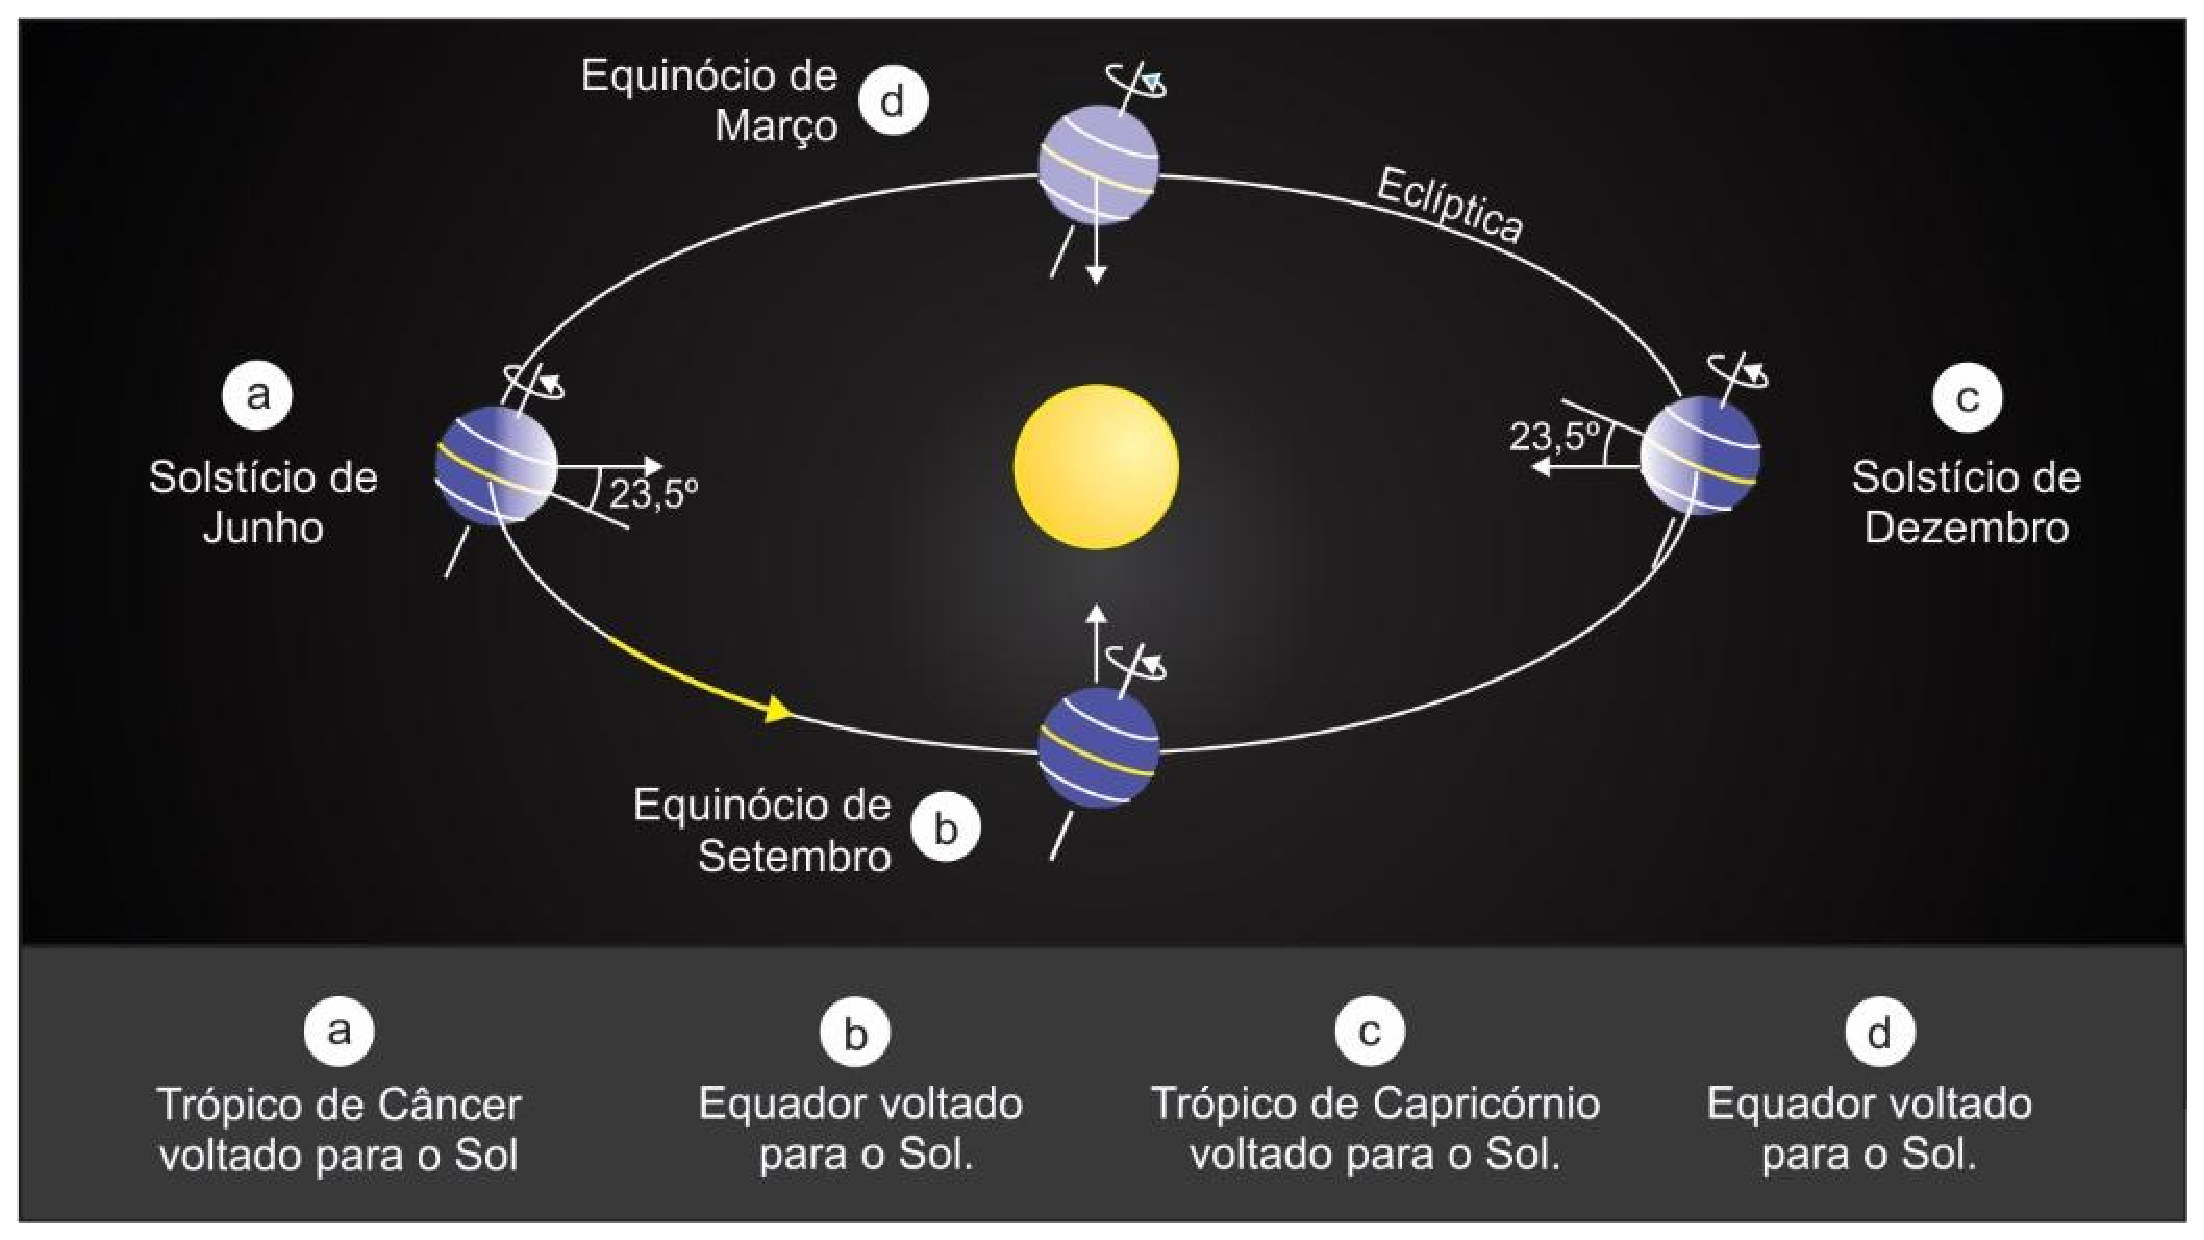
\includegraphics[keepaspectratio,scale=0.4,angle=0]{figuras/movimento.eps}
	\caption{Movimento da terra em torno do sol}
  \end{center}
\end{figure}

	Uma das formas de se observar a movimentação do Sol é através do gnômon, que é uma haste vertical fincada ao solo. Durante o dia a haste forma uma sombra onde o tamanho depende da época do ano e do dia do ano. A sombra é máxima no nascer do sol ou no pôr-do-sol e ela é mínima ao meio-dia. Ao longo do ano, à mesma hora do dia, a sombra é máxima no solstício de inverno, e mínima no solstício de verão.

\begin{figure}[H]
  \begin{center}
	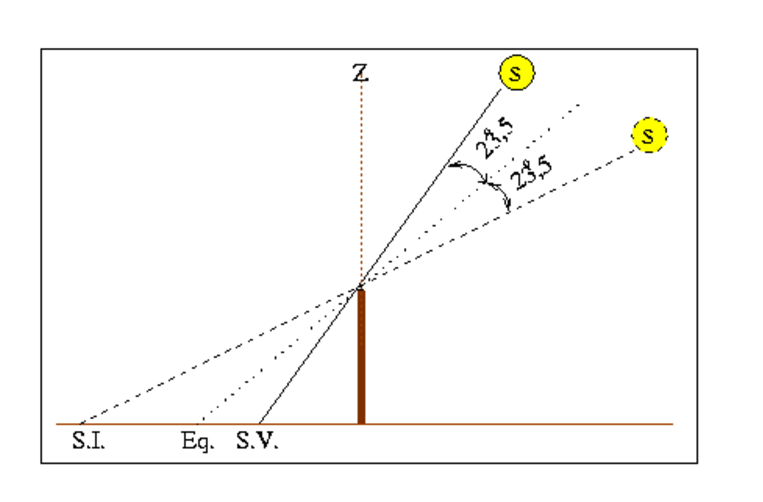
\includegraphics[keepaspectratio,scale=1,angle=0]{figuras/inclinacao.eps}
	\caption{Gnômon, S.I: Solstício de Inverno e S.V: Solstício de Verão}
  \end{center}
\end{figure}

	A partir do Gnomôn se registra numa carta solar a inclinação do sol conforme o horário e data, sendo que esta carta solar se aplica para toda a latitude correspondente, no caso de Brasilia verifica-se a carta solar referente à latitude de aproximadamente $16^o$ Sul\cite{2002Maciel}.

\begin{figure}[H]
  \begin{center}
	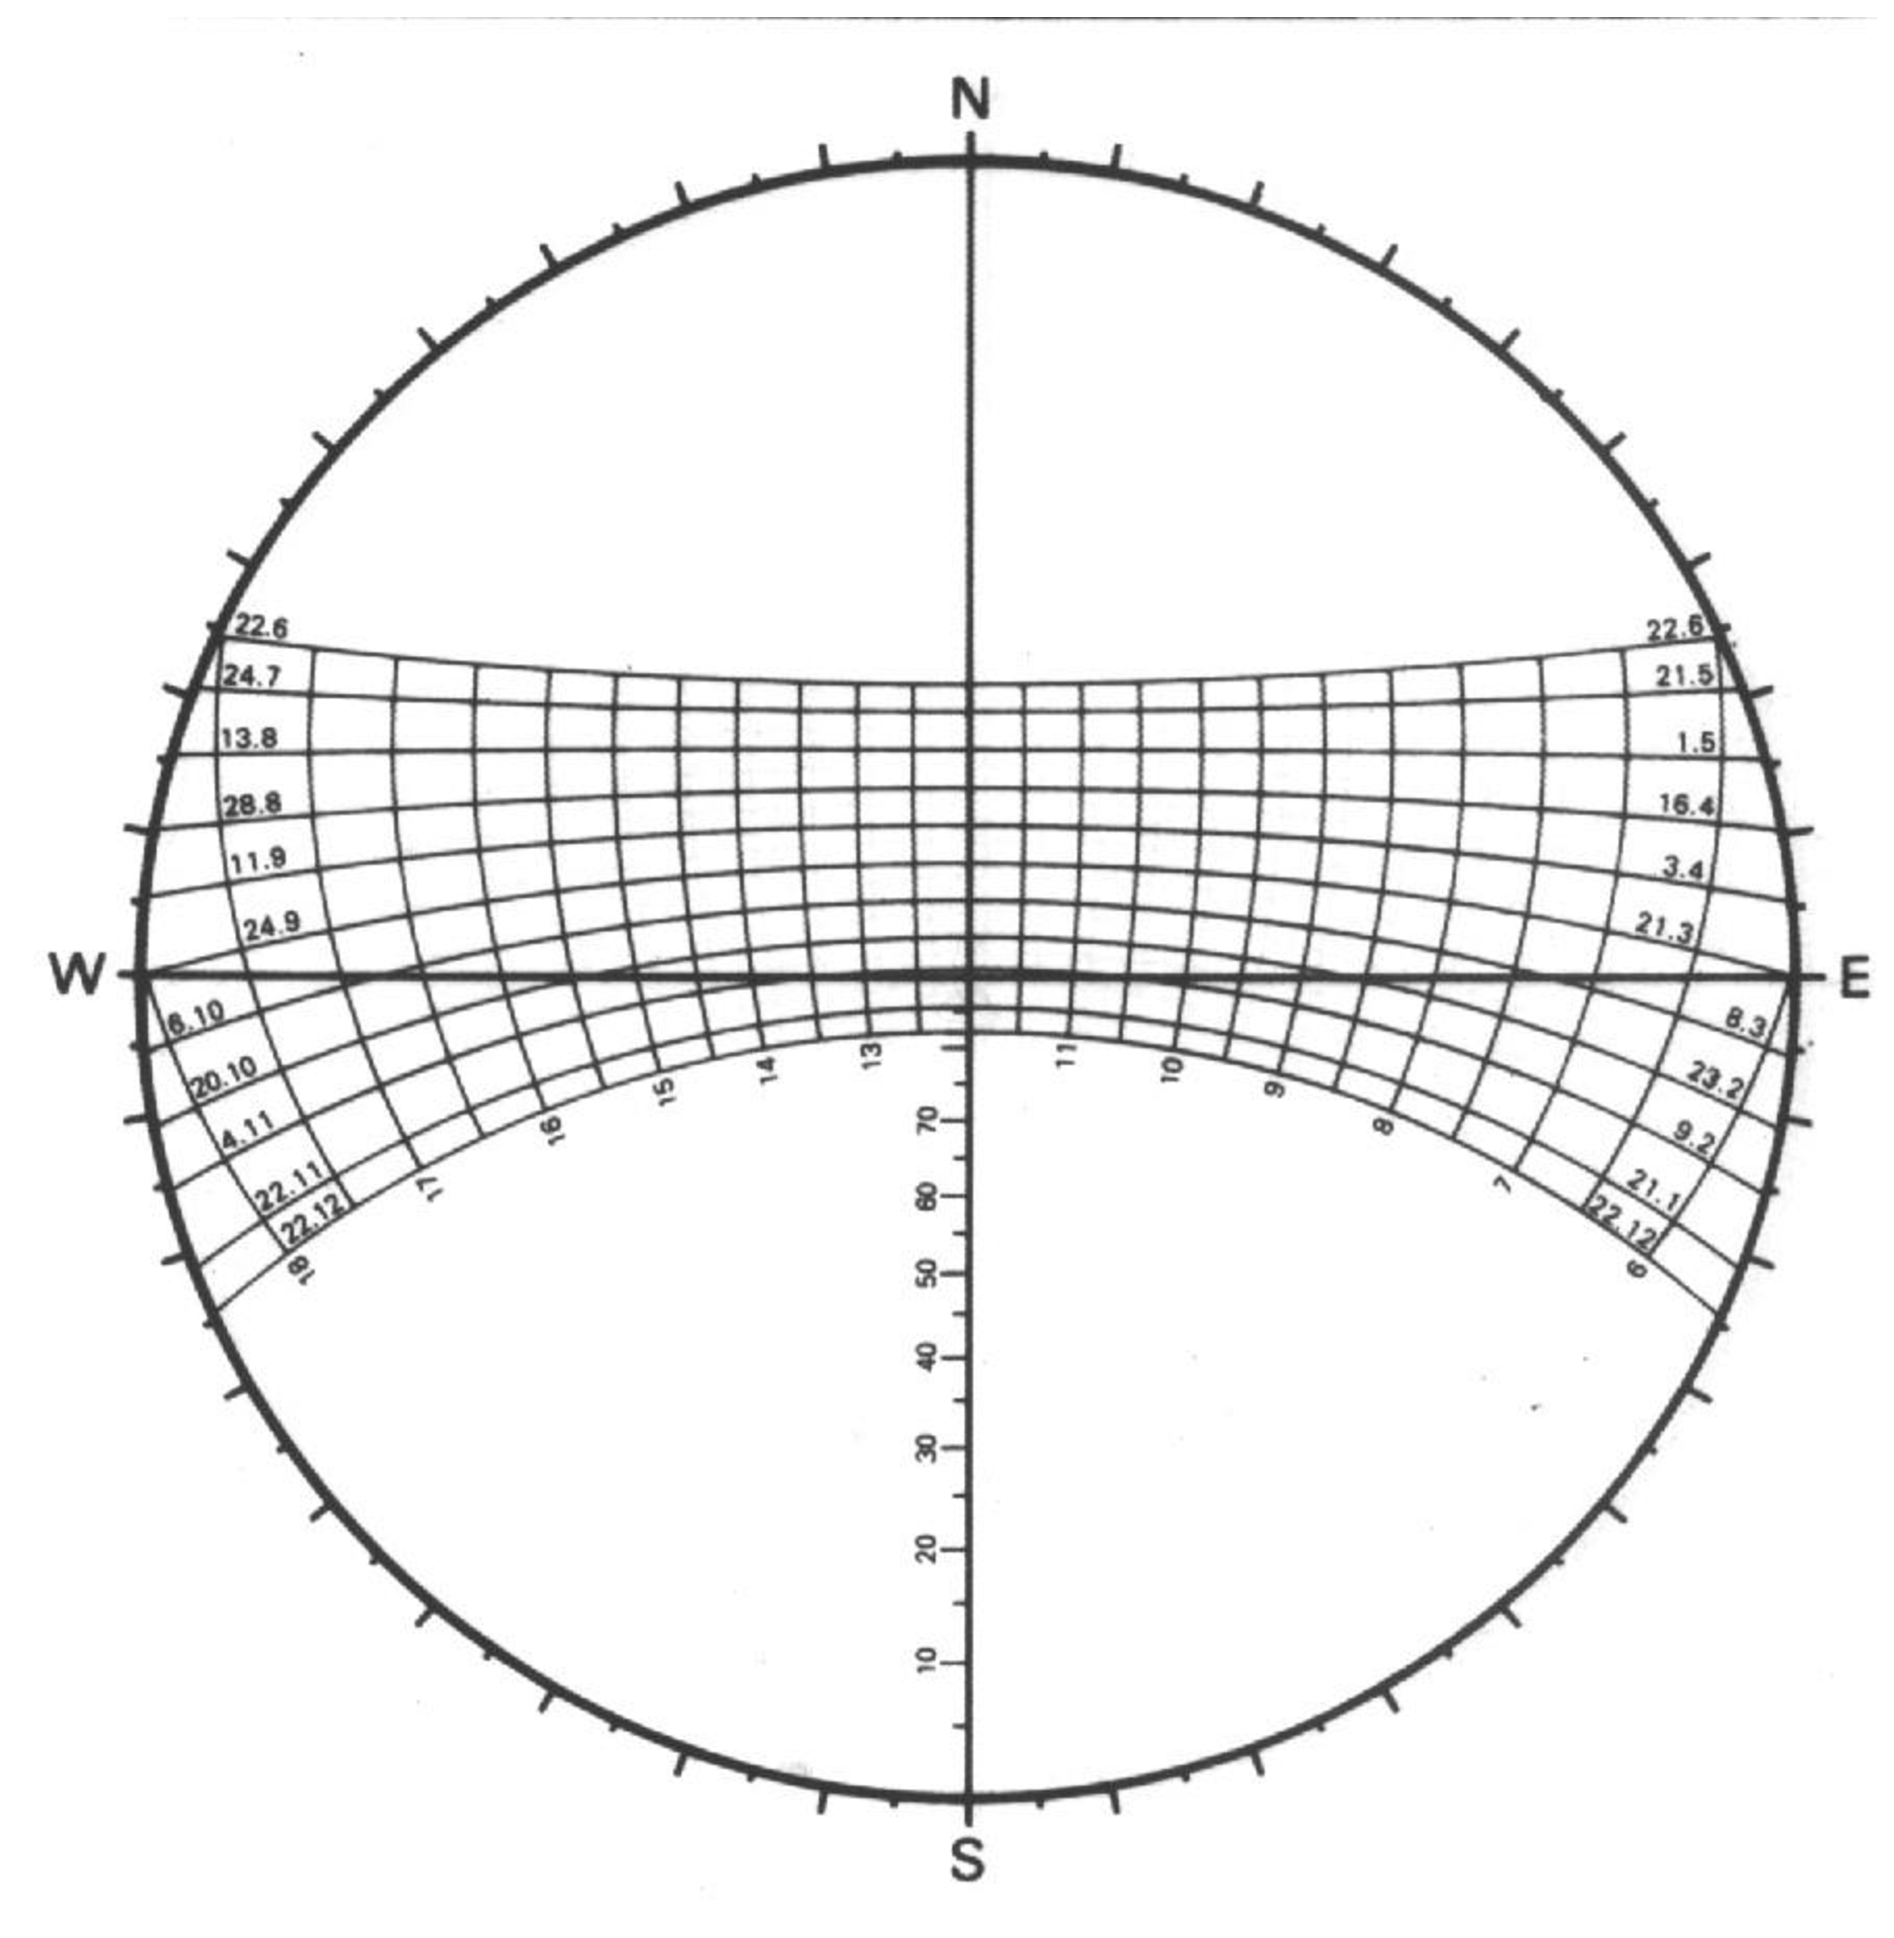
\includegraphics[keepaspectratio,scale=0.3,angle=0]{figuras/bioclimatico.eps}
	\caption{Carta solar de brasília}
  \end{center}
\end{figure}

\subsection{Ventos}

	No decorrer da estação chuvosa os ventos predominam o quadrante Norte, com variação NW (Noroeste)  e NE (Nordeste), no período os ventos mais fortes vêm de NW. A partir do mês de março predominam os ventos de direção E (Leste). No período de estiagem aumenta a incidência dos ventos de Sul e Sudeste.

	A tabela \ref{direcao_ventos}\cite{2015Instituto} mostra a direção dos ventos durante todo o ano:

\begin{table}[H]
\begin{tabular}{|c|c|c|c|c|c|c|c|c|c|c|c|}
\hline 
Jan & Fev & Mar & Abr & Mai & Jun & Jul & Ago & Set & Out & Nov & Dez\tabularnewline
\hline 
\hline 
NW & E & E & E & E & E & E & E & E & NE & NW & NW\tabularnewline
\hline 
\end{tabular}
\caption{Direção dos ventos durante o ano}
\label{direcao_ventos}
\end{table}

\section{Escolha dos Materiais Sustentáveis}

	Na escolha dos materiais devem ser consideradas a origem da matéria-prima, extração, processamento, gastos com energia para transformação, emissão de poluentes, biocompatibilidade, durabilidade, qualidade, entre outros que permitam classifica-los como sustentáveis ou ecológicos e elevar o padrão da obra no quesito de melhoria da qualidade de vida de seus habitantes e do próprio entorno. Essas características analisadas, devem estar de acordo com a geografia, tipologia, ecossistema, condições climáticas, resistência, responsabilidade social do ambiente onde será construído.

\subsection{Pisos - Ambiente Interno (Seco)}
	
	Caracteriza-se ambiente seco lugares onde não entram em contato com água frequentemente, como a sala, os quartos, escritórios e etc.

\subsubsection*{\textbf{Piso de bambu}}

	Em comparação com outras madeiras, o bambu tem crescimento muito rápido, com alta produtividade por hectare, além de ser altamente renovável e sustentável. O piso de bambu é mais forte, mais estável e mais durável do que a maioria dos pisos de outros tipos de madeira. Possui maior estabilidade dimensional e, portanto, menos expansão e contração do que pisos de madeiras tradicionais. A opção do piso de bambu traz um design à casa, o material está na moda no mercado e sua variedade de tonalidades que o próprio bambu tem aumenta o conforto do morador.


\subsubsection*{\textbf{Vantagens do bambu}}

	\begin{itemize}

		\item O bambu é relativamente forte e rígido

		\item O bambu pode ser cortado com ferramentas simples.

		\item A superfície do bambu é dura e limpa

		\item O bambu pode ser cultivado em pequena escala

		\item O retorno do capital é mais rápido do que se fosse usada madeira.

		\item As estruturas de bambu são flexíveis durante tormentas e terremotos

		\item O bambu pode ser usado com sucesso para reforçar um terreno deficiente, como por exemplo evitar desabamentos de terra ou para reforçar um caminho.
	\end{itemize}

\subsubsection*{\textbf{Desvantagens do bambu}}

	\begin{itemize}

		\item O bambu tem uma durabilidade natural baixa e necessita de tratamento

		\item O fogo representa um grande risco.

		\item Os talos do bambu não são totalmente retos, são estreitos. As emendas estão a distâncias diferentes e podem ser importunas quando se trabalha o material.

		\item A normalização é praticamente impossível devido à variação dos tamanhos.
	\end{itemize}

\subsubsection*{\textbf{Fábricas no Brasil}}

	\begin{itemize}

		\item \textbf{Ditzel} - Fabricante, Prudentopolis – PR

		\item \textbf{Lisonda} - Fabricante, Taboão da Serra - SP

		\item \textbf{Alphenas Design} - Fabricante, Taboão da Serra – SP

	\end{itemize}

\subsubsection*{\textbf{Preço}}

	O preço da ripa de bambu nas medidas 7mm x 18,7cm x 1,34m [$\si{\meter}^2$] está entre $R\$ 30,00$ e $R\$ 44,08$.

\subsubsection*{\textbf{Porque não usar outros tipos de madeira?}}
	
        Os critérios da escolha do material levam em consideração a forma de extração da matéria-prima do produto, e entre as opções o bambu tem uma maior velocidade de recuperação por metro quadrado (\si{\meter}$^2$), por conta disso, o bambu não tem grandes problemas com extinção. Mas, deve-se ficar atento se o bambu foi extraído de forma correta.

\subsection{Piso – Ambiente externo (Molhado)}

        Caracteriza-se ambiente molhado lugares que entram em contato com água frequentemente, como banheiros, área de serviços, entre outros.

\subsubsection*{\textbf{Piso Cerâmico}}

	No processo produtivo da cerâmica há reaproveitamento de sobras no próprio processo produtivo reduzindo os impactos ambientais, como o uso da água e argila por exemplo.

\subsubsection*{\textbf{Vantagens}}

	\begin{itemize}

		\item \textbf{Durabilidade}
		
		O piso cerâmico é muito mais durável que outro tipo de pisos. É também muito resistente à água e bactérias, sendo por isso uma boa opção para quem sofra de problemas respiratórios ou alergias. Devidamente instalado, o piso de cerâmica por durar por 20 anos ou até mais.

		\item \textbf{Variedade de modelos}
		
		O piso cerâmico pode ser encontrado em diversas cores, desde as mais vibrantes aos tons mais sóbrios. Alguns modelos de pisos cerâmicos apresentam também textura ou imitam, inclusive, pisos considerados mais nobres, como madeira ou mármore. Como este tipo de piso é vendido à peça, é possível criar padrões elegantes ou mais originais, dependendo da forma como são dispostas as telhas no chão.

		\item \textbf{Isolamento}
		
		Em climas mais secos e quentes, o piso cerâmico ajuda a manter a temperatura ambiente mais fresca.

		\item \textbf{Preço}
		
		Uma vez que o piso cerâmico é mais durável, o seu valor é considerado um bom investimento face a outros tipos de piso mais caros.

		\item \textbf{Instalação}
		
		A própria de instalação também fica mais econômica, sendo também muito simples de ser feita.

		\item \textbf{Fácil manutenção}
		
		Este tipo de piso tem uma manutenção muito simples, para além de ser muito fácil de limpar. Para o manter bonito e nas melhores condições basta simplesmente varrer o chão, limpando de seguida com um esfregão úmido e um pouco de detergente doméstico suave.

	\end{itemize}

\subsubsection*{\textbf{Desvantagens}}

	\begin{itemize}

	\item \textbf{Isolamento}

	Embora o piso cerâmico seja ideal para climas mais quentes, visto dar frescura ao ambiente, em climas mais frios pode tornar-se demasiado gelado quando em contato com os pés.

	\item \textbf{Escorregadio}
	
	Quando molhado este tipo de piso pode levar a quedas e fraturas, uma vez que se torna muito escorregadio. É por isso aconselhável que esteja bem seco antes de alguém o pisar.

	\item \textbf{Delicado}
	
	Durante a sua instalação o piso cerâmico pode ser muito delicado, podendo inclusive partir-se com alguma facilidade, quando não são tidos todos os cuidados necessários para a sua correta colocação no chão.

	\item \textbf{Superfície dura}
	
	Ao contrário de outro tipo de pisos, como o piso em carpete, o piso cerâmico apresenta uma superfície muito dura. Em casas com crianças pequenas é aconselhável que se utilize tapetes nas zonas de maior passagem e brincadeiras, para que exista uma superfície mais fofa no caso de quedas.

	\end{itemize}

\subsubsection*{\textbf{Fábricas no Brasil}}

	\begin{itemize}

	\item \textbf{Itagres} - São Cristóvão - Tubarão – SC

	\item \textbf{Portobello S.A.} - Tijucas - SC – Brasil

	\end{itemize}

\subsubsection*{\textbf{Preço}}
	
	O preço no mercado da cerâmica $48\times48 c\si{\meter}^{2}$ está entre $R\$ 10,90$ à $R\$ 16,22$.

\subsubsection*{\textbf{Porque não usar outros tipos de pisos?}}

	O piso cerâmico é de fácil limpeza, ou seja, em ambientes com constante contato com água ele se torna mais fácil de secar e limpar, além de deixar o ambiente mais refrescado e aconchegante, pelo contrário dos pisos de cimento queimado e pisos de borracha, onde o excesso de água prejudica a conformidade dos mesmos. O piso cerâmico entra nos critérios escolhidos pois na sua fabricação, todos os resíduos gerados nas etapas de extrusão, corte e laminação são reinseridos no processo de fabricação, reduzindo assim a quantidade de água e argila no processo de produção.


\subsection{Paredes - Tijolo Ecológico }

\subsubsection*{\textbf{Solo-cimento}}
	
	Solo-cimento é o material obtido pela mistura de solo, cimento e água. O tijolo deste material é feito pela prensa, manual ou automatizada, dessa mistura. Após a prensa ele passa pela cura e secagem, não sendo necessária sua queima, que lançaria resíduos tóxicos no meio ambiente, enquanto no processo tradicional é feito a queima do tijolo logo após a saída da prensa. Portanto, no processo da queima no tijolo tradicional, há emissões de gases como Dióxido de Carbono (CO$_2$), Dióxido de Enxofre (SO$_2$), Monóxido de Carbono (CO), Gases Oxidantes, Óxidos Nitrogenados e Compostos de Chumbo, gases esses que contribuem para o aquecimento global e poluição do ar\cite{1980PORTLAND}.\\

\subsubsection*{\textbf{Vantagens}}
	
	\begin{itemize}
		\item Seu modelo de produção é por meio da prensa hidráulica ou eco manual, onde a pressão exercida é de 6 toneladas, tornando-o regular, com faces lisas e que proporcionam um encaixe perfeito, viabilizando assim uma maior precisão também no cálculo de tijolos necessários na obra;

		\item A utilização dos tijolos ecológicos evita a necessidade do uso de materiais como arame, madeira, pregos e folhas de parede pronta para a instalação da rede elétrica, hidráulica etc;

		\item Possui isolamento acústico e térmico, o que possibilita tanto o aquecimento como o resfriamento do ambiente de maneira natural;

		\item Reduz a umidade nas paredes;

		\item Além de aumentar a resistência da estrutura, facilita toda a construção, uma vez que seu molde permite o encaixe fácil e rápido, sem a necessidade de utilização de gesso ou azulejos;

		\item Diferentemente dos tijolos tradicionais, os ecológicos necessitam de pequenas quantidades de cimento, dentre outros.

	\end{itemize}

\subsubsection*{\textbf{Desvantagens}}

	\begin{itemize}

		\item Requer pedreiro qualificado, com conhecimento da técnica de aplicação;

		\item Apesar de funcionar perfeitamente bem em climas secos, os tijolos ecológicos, quando aplicados em locais de climas úmidos ou de maior exposição à umidade, ainda não é totalmente indicado.

	\end{itemize}

\subsubsection*{\textbf{Fábricas no Brasil}}

	\begin{itemize}

		\item \textbf{PERMAQ} - São Paulo - SP – Brasil

		\item \textbf{Monteiro Tijolos} - Salto – SP

		\item \textbf{Sete Tijolos Ecológicos} - Campo Grande/MS

	\end{itemize}

\subsubsection*{\textbf{Preço}}

	Nas medidas de $25 cm \times 12,5 cm$ e $6,5 cm$ de altura está entre $R\$ 1,00$ à $R\$ 1,20$ a unidade.

\subsubsection*{\textbf{Porque trocar o tijolo convencional por tijolo ecológico?}}

	O tempo de construção com o tijolo ecológico é muito menor, devido aos encaixes que favorecem o alinhamento da parede. A estrutura é mais segura pois as colunas são embutidas nos furos, e a sua carga de peso é melhor distribuídas. O tijolo ecológico tem uma durabilidade que chega a seis vezes maior que a dos tijolos convencionais, além de isolamento térmico e acústico gerados pelos furos no meio dos tijolos, que formam câmaras de ar e por fim as instalações hidráulicas e elétricas podem ser realizadas através dos furos. Como já dito anteriormente, o tijolo ecológico entra nos critérios de escolha de materiais pela forma em que se é produzida, gerando menos resíduos e impactos ambientais na sua fabricação comparado com os tijolos convencionais.

\subsection{Tinta - Ambientes Internos e Externos }

\subsubsection*{\textbf{Tinta Mineral Natural}}
	
	Conhecida também como tinta mineral ecológica, é feita na base de terra crua e emulsão aquosa. Tal matéria prima é retirada de jazidas certificadas\cite{EcoCasa}.

\subsubsection*{\textbf{Vantagens}}
	
	\begin{itemize}

		\item Não agride o meio ambiente

	As tintas minerais naturais são não tóxicas, e não prejudicam o meio   ambiente. Além disso, seu preparo e confecção e processo produtivo configuram fatores ecologicamente corretos.

		\item Não possui nenhum tipo de Composto Orgânico Volátil (COVs – reconhecido como um perigoso poluente)

	Os COVs são nocivos para o meio ambiente. Sua evaporação agride a camada de ozônio.Os produtos que contém esses compostos afetam a saúde, pois sua evaporação pode provocar problemas como irritação nas vias respiratórias, fadiga, falta de ar, dor de cabeça, náuseas, danos ao sistema nervoso, ao fígado, aos rins e câncer.
 
		\item Não possui biocidas, estabilizantes ou corantes
		
		\item Durável
		
		\item Lavável
		
		\item Contribui na manutenção de umidade relativa do ar e troca de calor
		
		\item Fácil aplicação e ótimo rendimento, dispensando qualquer base de preparo
 
	\end{itemize}

\subsubsection*{\textbf{Fábricas no Brasil}}

	\begin{itemize}

		\item \textbf{Kroten} - Pomerode - SC - Brasil - (47) 3395 0230 -

		\item \textit{Fábrica escolhida} \textbf{Solum} - Vila Madalena – SP,  Brasil -  (11) 3097-8716 

	\end{itemize}

\subsubsection*{\textit{Fábrica Escolhida} \textbf{Solum}}

\begin{longtable}{|m{7cm}|m{7cm}|}
\hline 
Fábrica Solum & Outras Fábricas\tabularnewline
\hline 
\hline 
Muitas informações online, facilitando a pesquisa e a escolha & Menos informações, dificultando o conhecimento sobre o produto, e
consequentemente sua escolha\tabularnewline
\hline 
Possui uma paleta de 20 cores, o suficiente para a maioria dos usos
da casa & Algumas possuem pouca quantidade de cores, não sendo viável sua escolha\tabularnewline
\hline 
O preço do galão se mantém na média & Algumas fábricas possuem o preço muito acima da média\tabularnewline
\hline 
\caption{Vantagens da Solum sobre outras fábricas}
\end{longtable}

\subsubsection*{\textbf{Características Técnicas}}
	
	\begin{itemize}
		
		\item \textbf{Composição}
		
		Pigmentos de terra, água, emulsão base água e cargas minerais.
		
		\item \textbf{Embalagem}
		
		Baldes de 18 litros e 10 litros.
		
		\item \textbf{Rendimento da pintura}
		
		1 Litro/$\si{\meter}^{2} = 18\si{\meter}^{2}/$balde, com 2 demãos superfície acabada.
		
		\item \textbf{Rendimento do revestimento}
		
		1,4 Litro/$\si{\meter}^{2} = 13\si{\meter}^{2}/$balde, com 2 demãos superfície acabada.
		
		\item \textbf{Validade}
		
		90 dias da data impressa no balde.
	
	\end{itemize}

\subsubsection*{\textbf{Preço}}

	Preço do balde de 18 litros = $R\$ 255,00$


\subsection{Madeira (Áreas Externas) }

\subsubsection*{\textbf{Madeira Plástica Ecológica}}
	
A madeira plástica vem como uma opção sustentável para o uso da madeira em ambientes externos (decks, piers e outros). O produto é resultante de matérias-primas recicláveis, por exemplo resíduos plásticos industriais variados\cite{EcoCasa}. É totalmente reciclado e reciclável, além de ser composto de material completamente sustentável\cite{ReWood}.

\subsubsection*{\textbf{Vantagens}}
	
	\begin{itemize}
		\item Zero de manutenção
		\item Totalmente feita de resíduos plásticos.
		\item Resistência à umidade;
		\item Resistência mecânica;
		\item Imunidade a pragas;
		\item Resistência à intempérie;
		\item Dispensa qualquer tipo de manutenção;
		\item Não degrada;
		\item Dispensa a pintura com vernizes e tintas.
	\end{itemize}

\subsubsection*{\textbf{Produtos que podem ser obtidos com o uso de madeira plástica}}
	
	\begin{itemize}
		\item Decks
		\item Bancos 
		\item Lixeiras para áreas externas
		\item Assoalhos
		\item Fachadas
		\item Pergolado
	\end{itemize}

\subsubsection*{\textbf{Fábricas no Brasil}}
	
	\begin{itemize}
		\item \textbf{Ecopex} - Jandira - SP, Brasil - (11) 4181 1103
		\item \textbf{In Brasil} - São Gabriel União da Vitória - Paraná - (42) 3522-1771
		\item \textbf{ReWood} - (11) 2402-4230
	\end{itemize}

\subsubsection*{\textit{Madeira Escolhida} \textbf{ReWood}}

\begin{longtable}{|m{7cm}|m{7cm}|}
\hline 
Madeira Plástica ReWood & Outras Madeiras Plásticas\tabularnewline
\hline 
\hline 
Tem aparência e textura de madeira natural, além de ser antiderrapante. & Algumas podem se assemelhar ao plástico, logo, tendo uma aparência mais artificial e textura mais lisa, o que faz ser mais derrapante que a madeira da rewood e a própria madeira natural.\tabularnewline
\hline 
Absorve pouca temperatura & Absorve muita temperatura\tabularnewline
\hline 
Garantia de 10 anos & Garantias não ultrapassam 3 anos\tabularnewline
\hline 
\caption{Vantagens da ReWood sobre outras madeiras plásticas}
\end{longtable}

\subsubsection*{\textbf{Preço}}

	$R\$199,90$ cada metro quadrado, sem a necessidade de manutenção futura\cite{BlogReWood}.

\subsection{Portas e Janelas}

\subsubsection*{\textbf{Tamanhos médios}}

	\begin{itemize}
	\item \textbf{Portas}

	de entrada: $1,02 \times 2,10 \si{\meter}$.

	banheiros e quartos: $0,72 \times 2,10 \si{\meter}$.

	áreas de circulação: $0,92 \times 2,10 \si{\meter}$.


	\item \textbf{Janelas}

	quartos: $1,20 \times 1,20 \si{\meter}$.

	banheiros: $0,60 \times 0,60 \si{\meter} e 0,60 \times 0,80 \si{\meter}$.

	\end{itemize}

\subsubsection*{\textbf{Materiais}}
	
	Partindo dos materiais já definidos, foi possível determinar que a madeira plástica não pode ser utilizada para a confecção de portas, logo não será utilizada para esse fim. Além disso, não foram encontrados materiais totalmente ecologicamente conscientes ou totalmente sustentáveis para esse fim, logo, serão usados materiais comuns de construção para a definição dos mesmos.

	Com isso, foi definido que as janelas serão de vidro, com o tamanho médio definido anteriormente.

	E além disso, as portas de fora da casa serão também de vidro, e as portas de dentro, serão de madeira, todas com o tamanho médio definido anteriormente\cite{2009Valente}.

\subsection{Telha}

\subsubsection*{\textbf{Telhas Ecológicas}}

	Produzidas a partir de fibras naturais ou materiais reciclados, As telhas ecológicas apresentam baixo custo de produção e podem ser utilizadas com as mesmas aplicações das telhas convencionais, 

\subsubsection*{\textbf{Vantagens}}

	\begin{itemize}

		\item Fácil manuseio e instalação: seu estoque e transporte são fáceis (pois a telha é flexível) e reduzem o número de quebras / perda de material (é recomendado que seja utilizada mão-de-obra especializada);
		\item Economia de tempo e material: a maioria é mais leve que a telha tradicional, reduzindo os custos da construção (a estrutura é mais leve e o serviço é realizado rapidamente). É importante destacar que o planejamento é essencial para a redução dos custos, ou seja, o desenvolvimento de um bom projeto arquitetônico e estrutural é essencial, decidindo quais materiais e acabamentos serão utilizados antes mesmo de iniciar a obra;
		\item É um material resistente: são resistentes e flexíveis, resistindo a chuvas de granizo;
		\item A maioria não propaga chamas;
		\item São impermeáveis: absorvem muito menos água do que as telhas convencionais e geralmente seu acabamento evita a proliferação de limo;
		\item Promovem o conforto térmico: alguns tipos ajudam a criar um ambiente interno mais confortável (menos quente);
		\item Design: é possível encontrá-las em vários formatos e cores (inclusive pigmentada dos dois lados permitindo ser instalada sem forro). Além disso é possível pintá-las com tintas à base de água;
		\item São sustentáveis: geralmente produzidas com fibras e resinas, materiais reciclados (como papel, caixa de leite longa vida) e não contém amianto (o qual é tóxico);
	
	\end{itemize}

\subsubsection*{\textbf{Fábricas no Brasil}}
	
	\begin{itemize}
	
		\item \textbf{GLZ} - Telhas e Laminados Ecológicos -Santa Cruz do Sul – RS
		\item \textbf{Eccoclean Telhas Ecológicas} - Saquarema – RJ
		\item \textbf{ECO-LÓGICA} - Vicente Pires/DF
		\item \textbf{Onduline} - Juiz de Fora/ MG
	\end{itemize}

\subsubsection*{\textbf{Preço}}

	Nas medidas $2,20\si{\meter} \times 0,95\si{\meter} \times 6\si{\meter\meter}$ à partir de $R\$ 9,50$.

\subsubsection*{\textbf{Porque não usar outros tipos de telhas?}}

	Entre os diversos tipos de telha, sobressaem duas: a telha de cerâmica e a telha ecológica. Os produtos feitos de cerâmica, tem grandes vantagens por sua produção reaproveitar os produtos não conformes, reduzindo os resíduos, o uso de água e argila, como já dito anteriormente. Já as telhas ecológicas, feitas a partir de camadas de vibras vegetais impermeabilizadas foi escolhido pois, ele é feito a partir de material reciclável, ou seja, o destino final de uma caixa de leite longa vida por exemplo, não é mais um aterro, e sim como matéria-prima para a fabricação de telhas ecológicas. Por conta disso, e de acordo com os critérios estabelecidos as telhas ecológicas foram escolhidas.

\subsection{Onde vai ser comprado?}

	Um dos critérios para a escolha dos materiais é levar em conta a localização do produto, logo os produtos vendidos em Brasília serão priorizados.


\subsubsection*{\textbf{Piso Cerâmico}}

	A fabricante Portobello tem filiais em todo Brasil, e em Brasília se encontra nos seguintes endereços: SAI Trecho 03, Lote 550 – SUL e SEUPN – Qd 509, Conj. B – Loja08/76 – Edifício Contag – Asa Norte.

\subsubsection*{\textbf{Tijolo Ecológico}}
	
	Uma loja de tijolos ecológicos em Brasília é a Ecoplanalto DF encontrada na Ceilândia Norte. CEP: 72215-000.

\subsubsection*{\textbf{Telha Ecológica}}

	A fábrica Eco-lógica tem sua sede na Chácara 167 – Lota 3$^a$ – Vila São José- Vicente Pires/DF. CEP: 73110-800.

\subsubsection*{\textbf{Piso de Bambu}}

	É o único produto que não há lojas em Brasília, logo a loja mais próxima é em São Paulo na Rua Princesa Isabel, 291 – Brooklin.


\section{Planta da Casa}

	A planta tem que ser planejada para que fatores ambientais como vento, sol, frescor das plantas e outros, sejam melhores aproveitados de forma a proporcionar conforto para os moradores.

	Analisando as necessidades do nosso projeto e da família para qual ele será construído, optamos por determinamos a nossa localidade no bairro Jardim Botânico, DF, e nos pautamos da média das casas desse setor e das famílias que lá residem para determinar a área útil da casa e a formação da família.

	Utilizamos como projeto base a planta baixa da “Casa Campo Grande”\cite{plantaCasa}, pois se mostra uma alternativa válida no quesito número de moradores e espaço disponível para construção, tendo $240\si{\meter}^{2}$ de área construída.

\begin{figure}[H]
  \begin{center}
	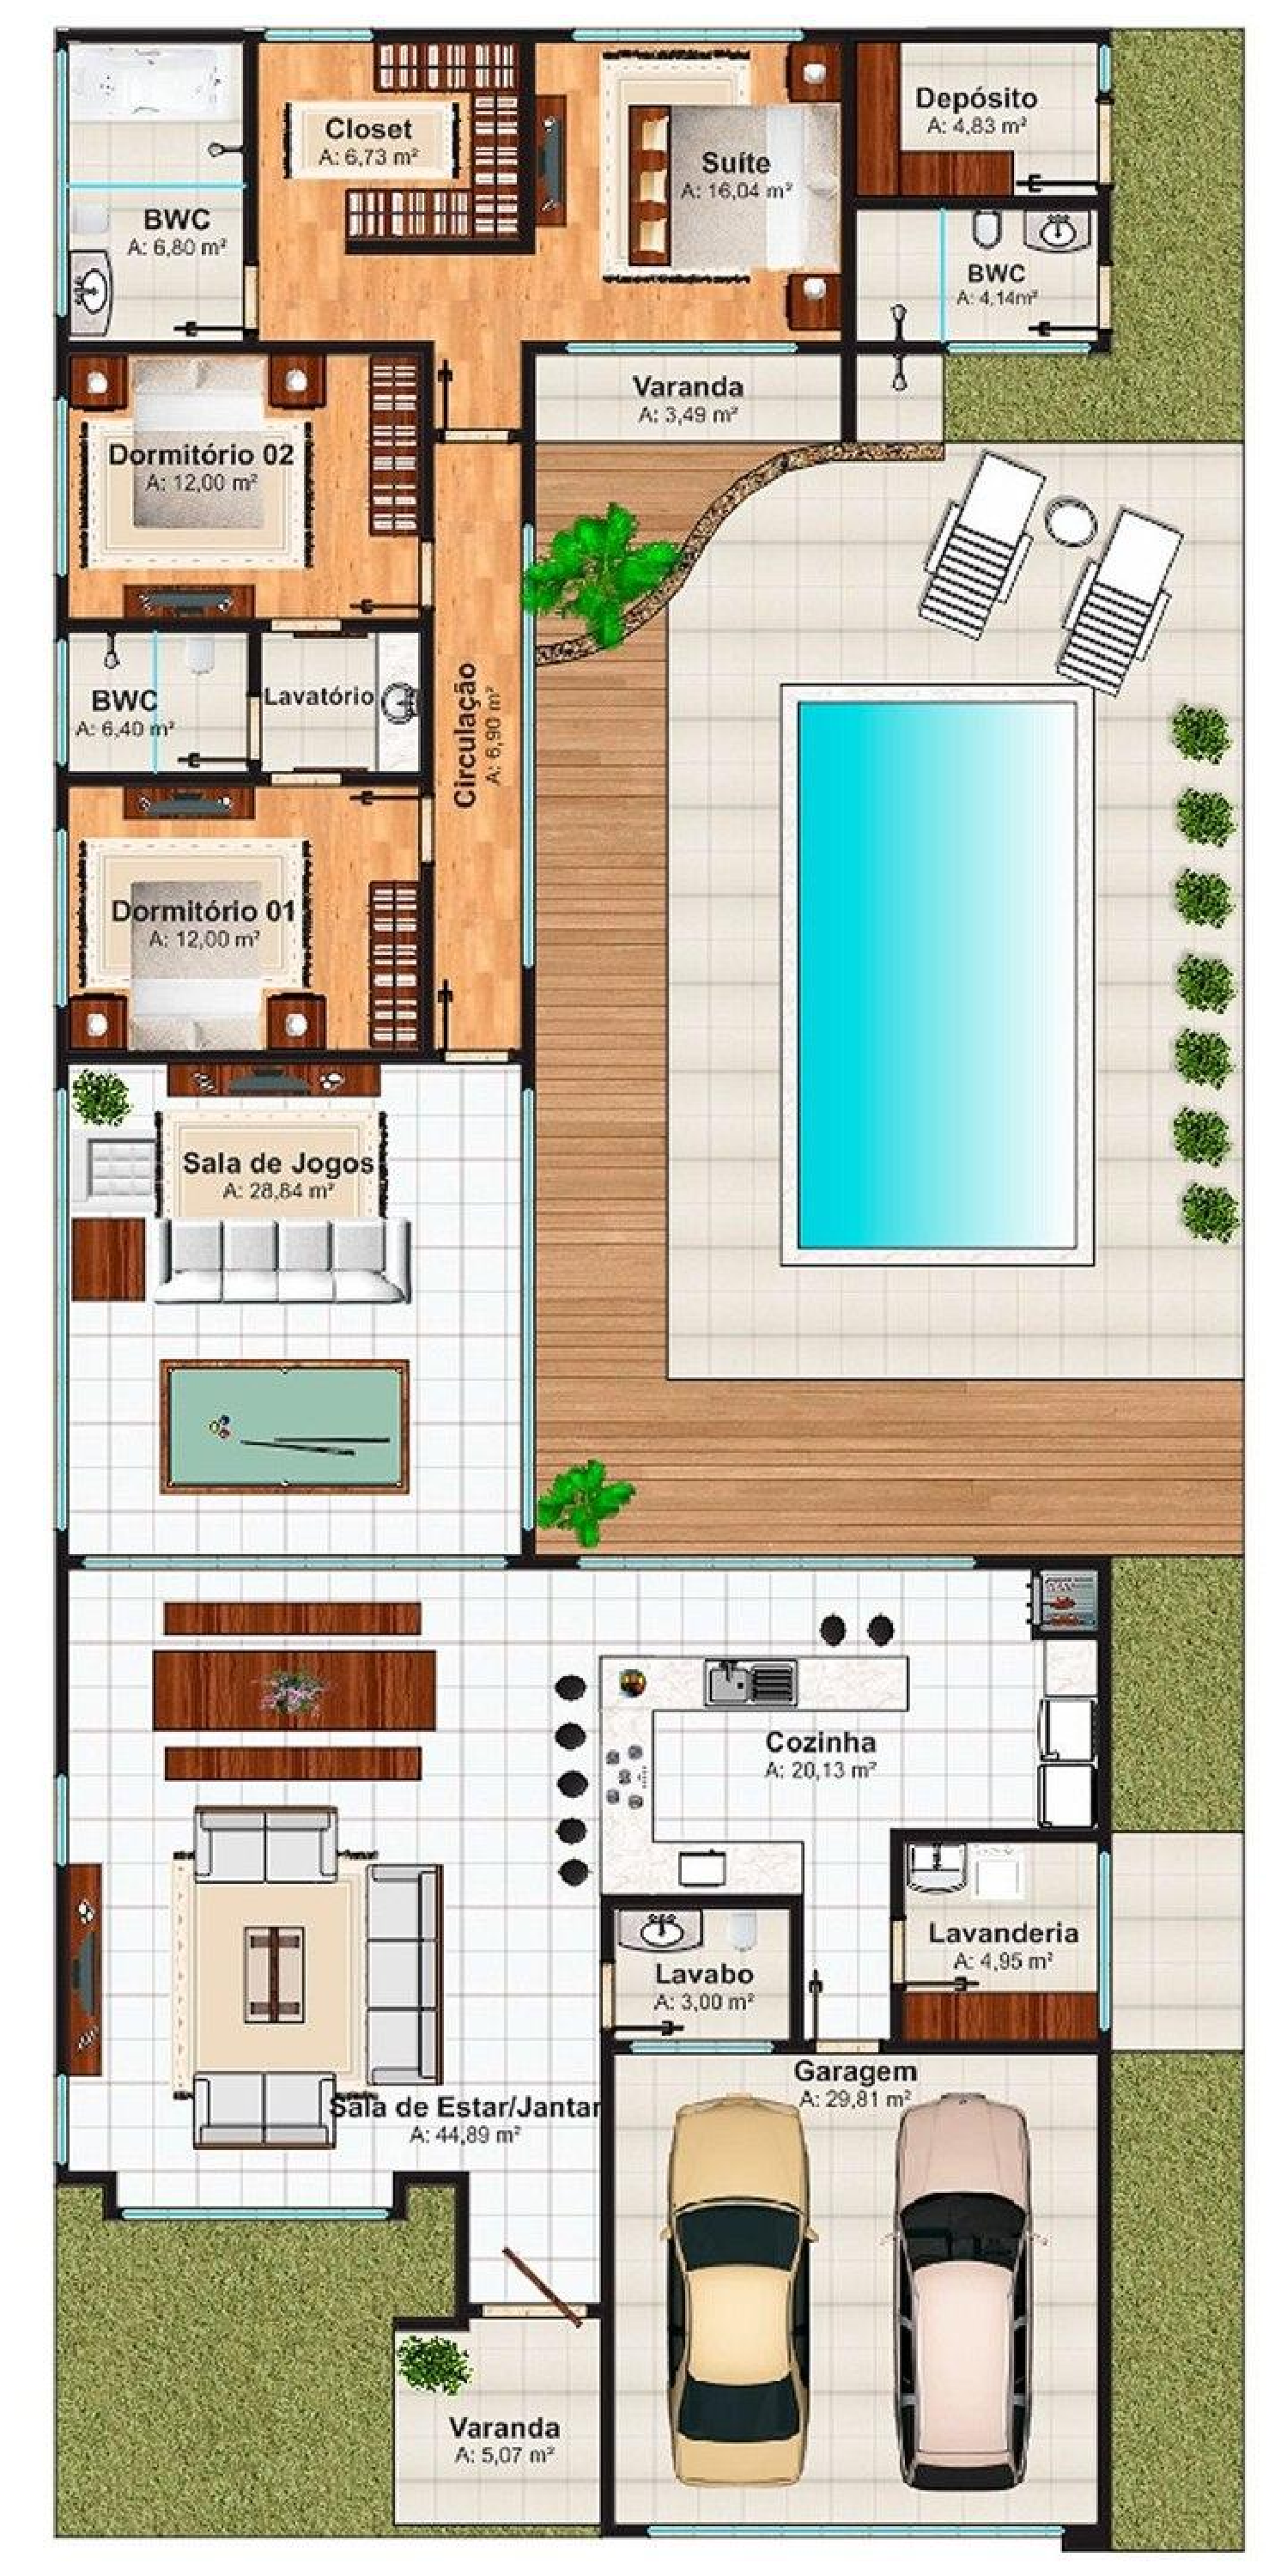
\includegraphics[keepaspectratio,scale=0.3,angle=0]{figuras/planta.eps}
	\caption{Planta da casa}
  \end{center}
\end{figure}


\begin{figure}[H]
  \begin{center}
	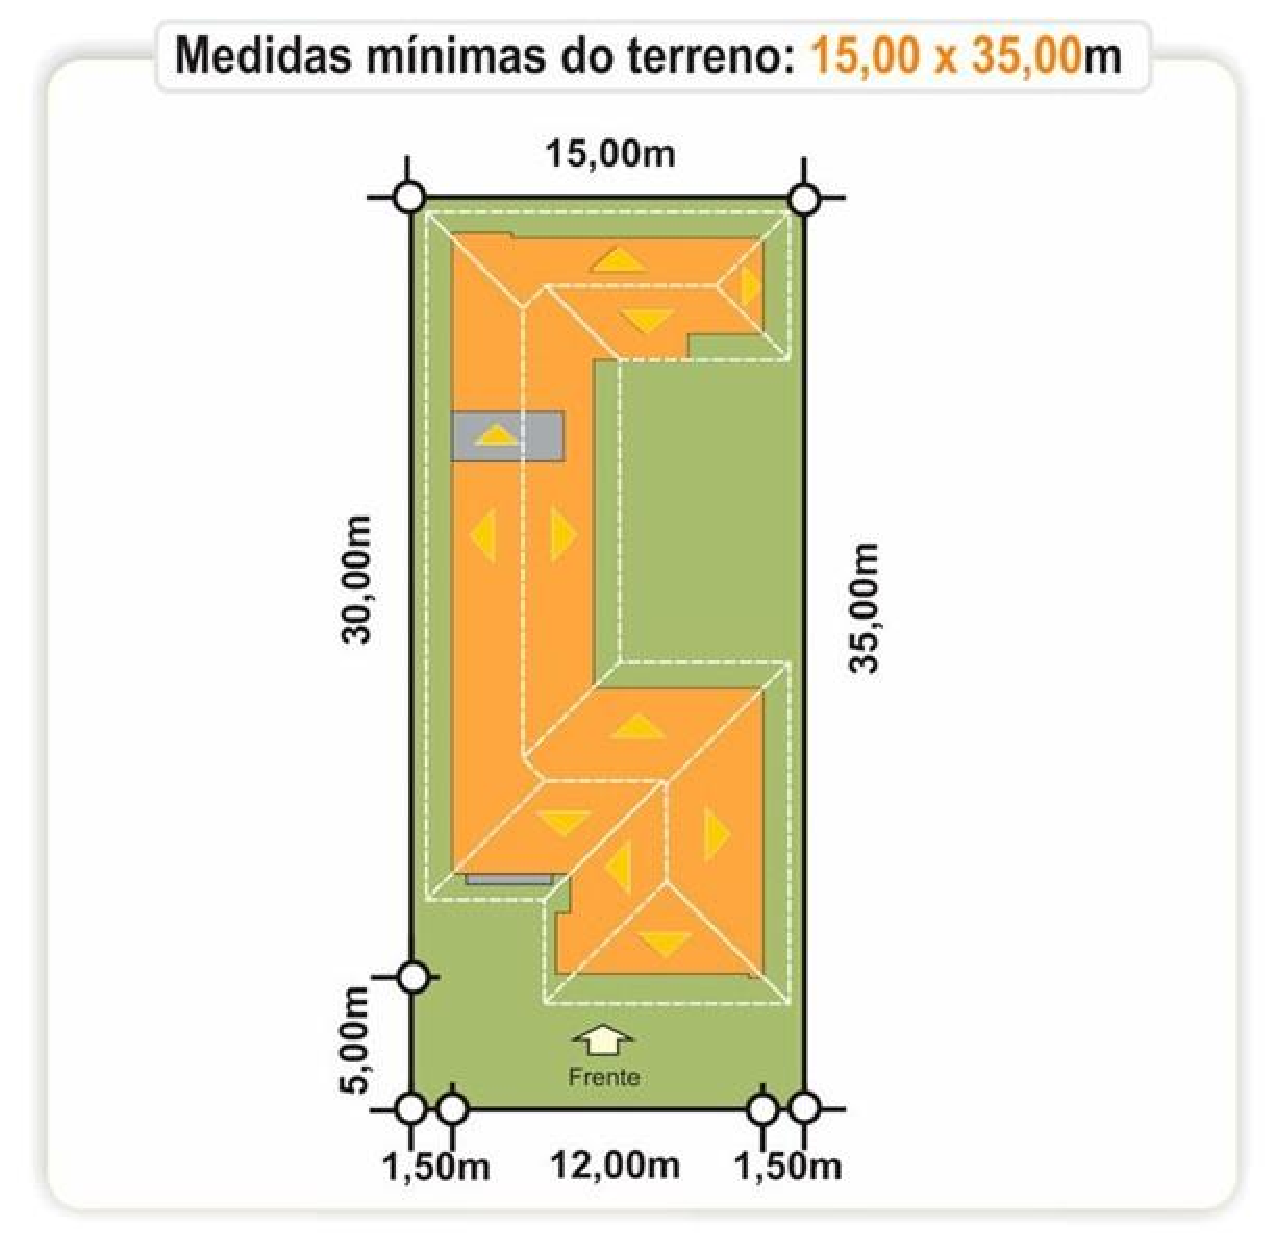
\includegraphics[keepaspectratio,scale=0.7,angle=0]{figuras/medidas.eps}
	\caption{Medidas da casa}
  \end{center}
\end{figure}

	Considerando as restrições do projeto base considerando as alterações feitas e aspectos de conforto térmico e maior eficiência das placas solares, determinou-se como possível localização da casa o Lote 3 do Conjunto N do Condomínio Jardim Botânico VI, de 15 metros de comprimento por 40 de largura, totalizando $600\si{\meter}^{2}$, sendo que a frente para a rua está posicionada para oeste.

\newpage

\begin{figure}[H]
  \begin{center}
	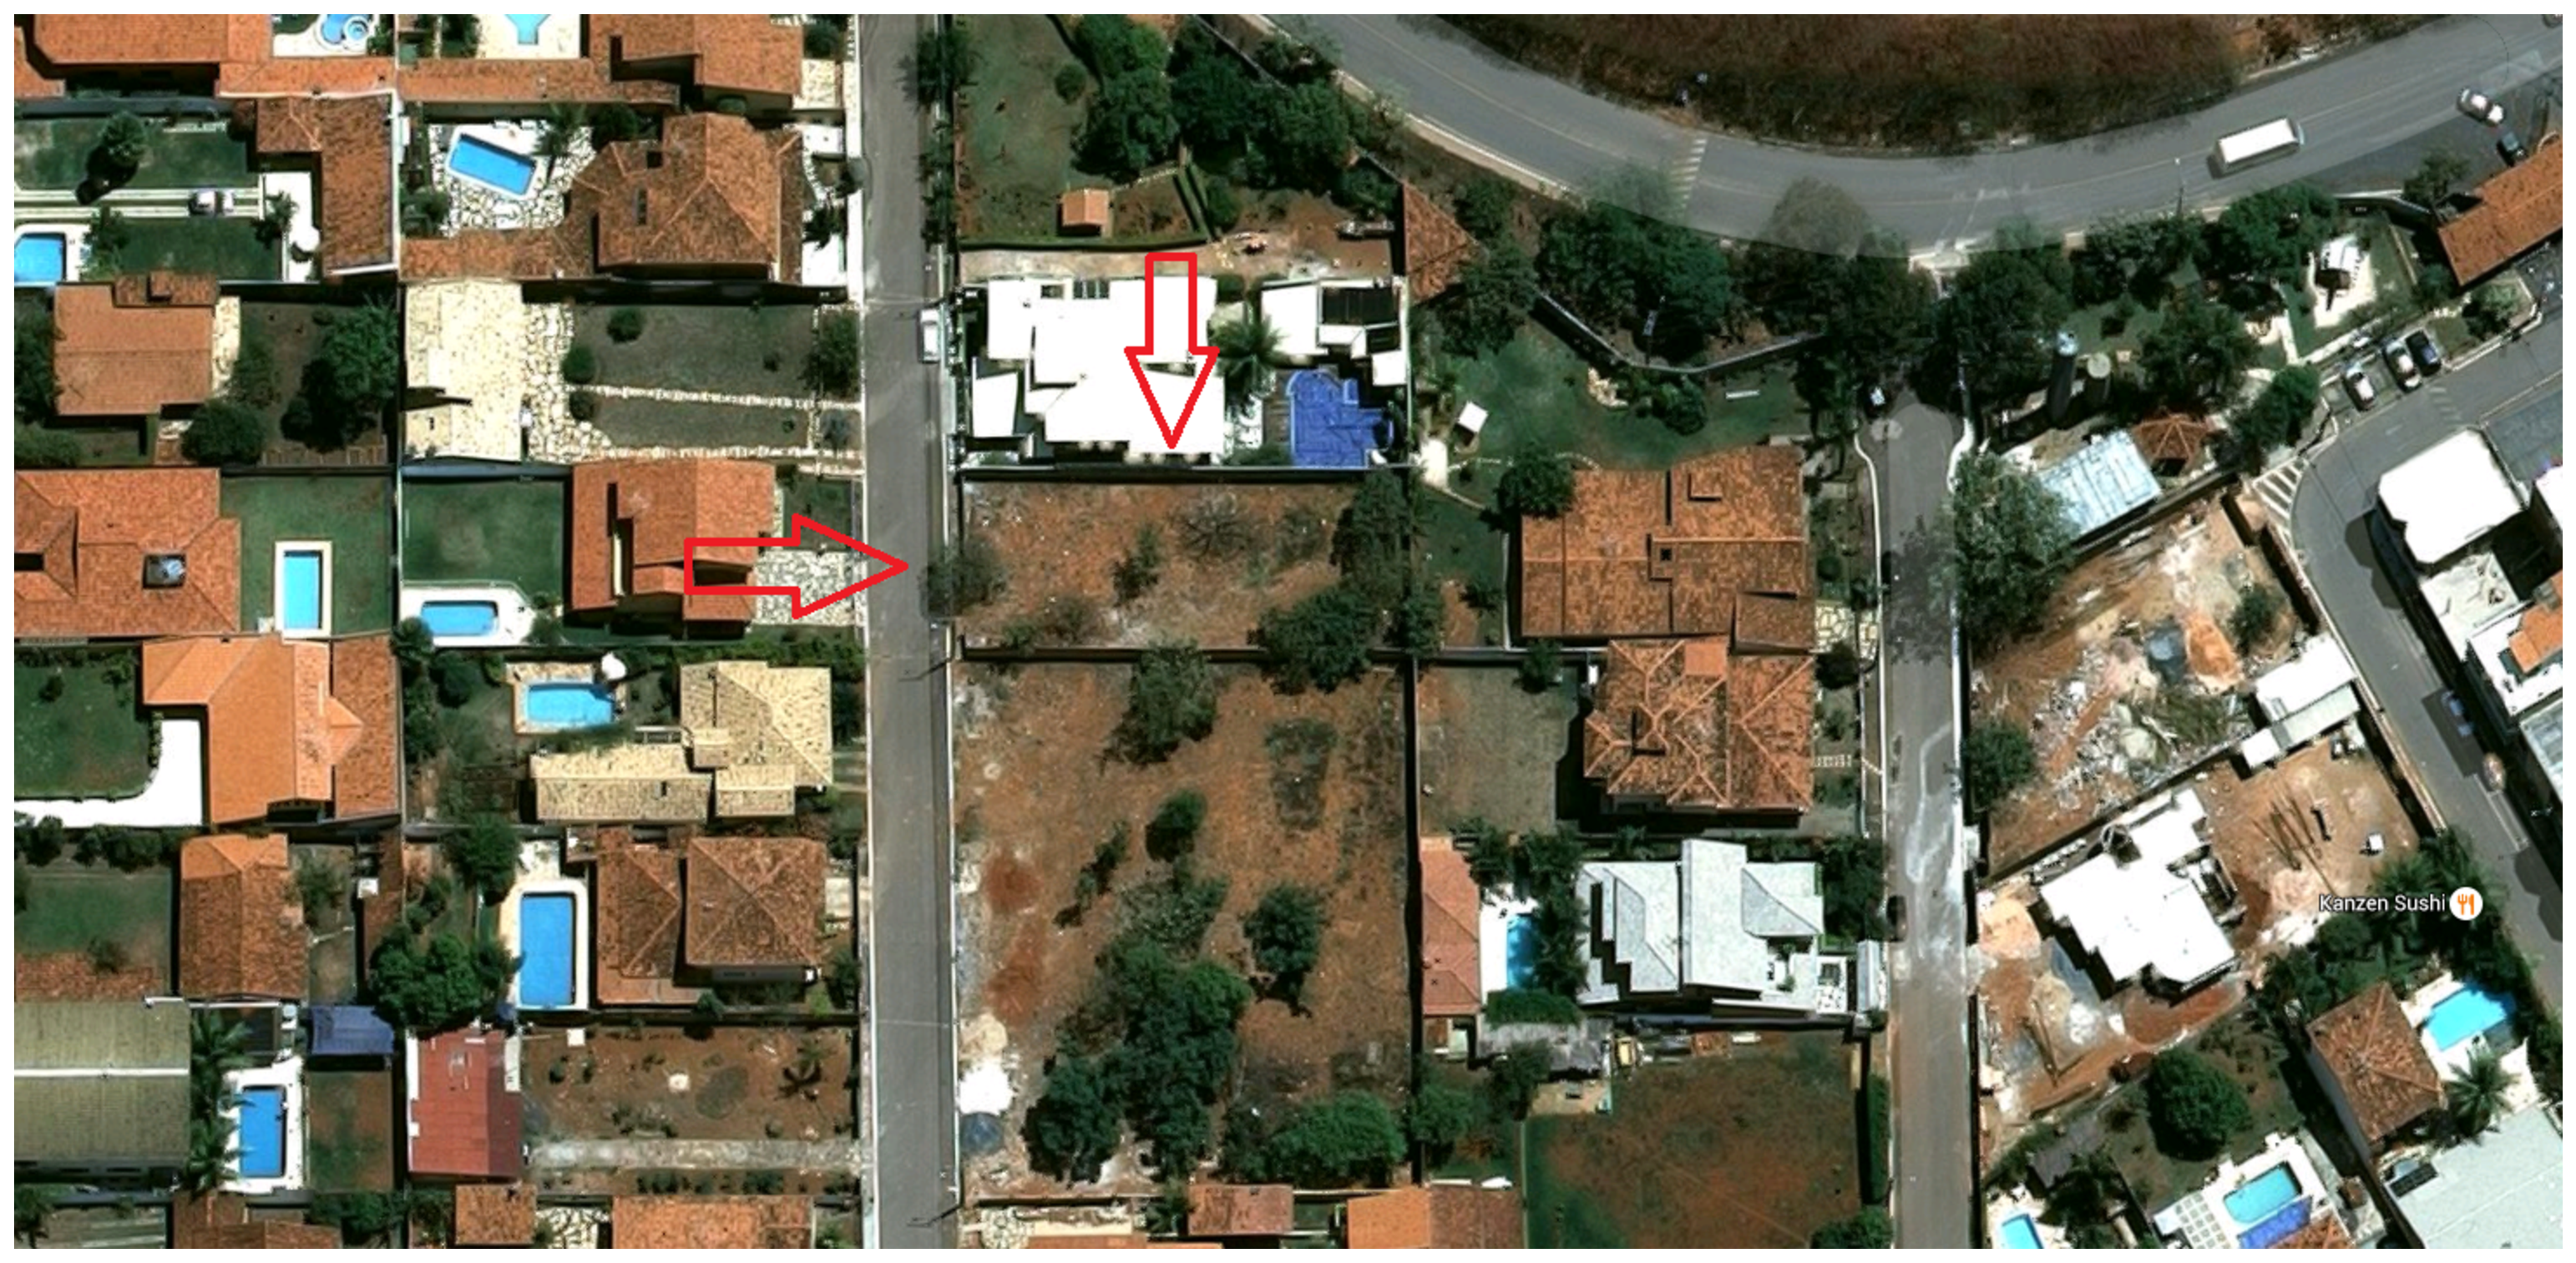
\includegraphics[keepaspectratio,scale=0.3,angle=0]{figuras/terreno.eps}
	\caption{Terreno da casa}
  \end{center}
\end{figure}

	Com base nos valores do último edital da Terracap\cite{TerracapJB}, foi calculado o valor médio do metro quadrado de um lote no Jardim Botânico.

$$\dfrac{292000}{802} = 364,09 \textup{ reais}/\si{\meter}^{2}$$
$$\dfrac{280000}{750} = 373,33 \textup{ reais}/\si{\meter}^{2}$$
$$\dfrac{364,09 + 373,33}{2} = 368,71 \textup{ reais}/\si{\meter}^{2}$$

Assim, o terreno escolhido com 600m² custa cerca de $R\$ 221.226,00$

\begin{figure}[H]
  \begin{center}
	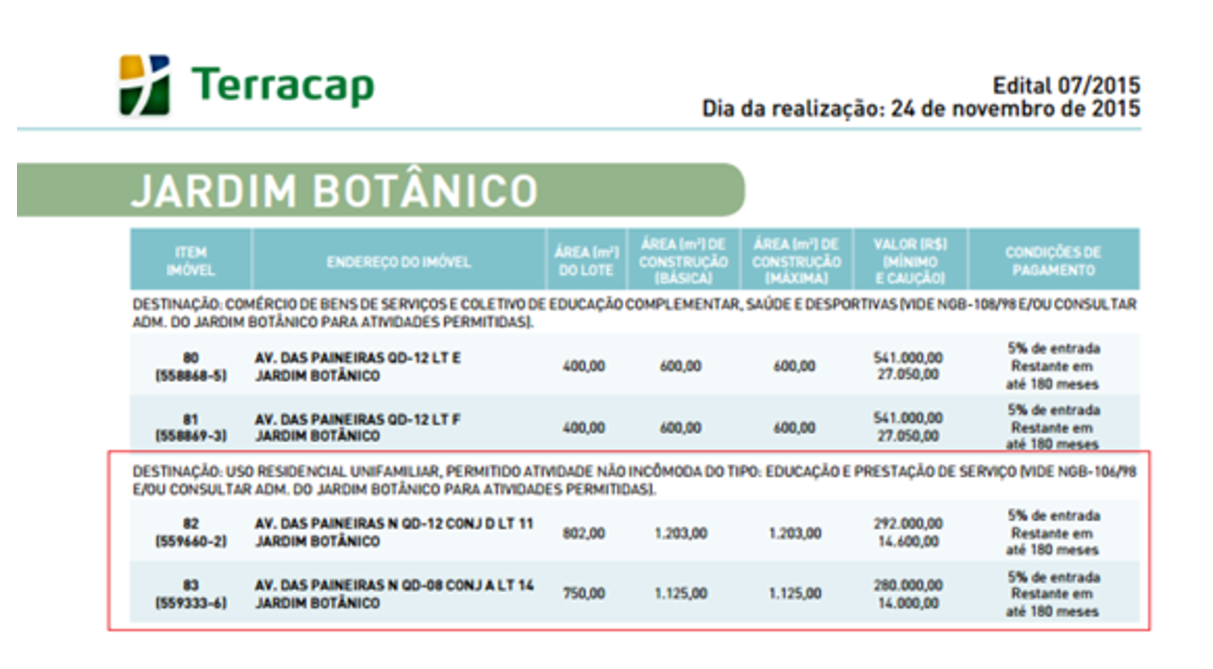
\includegraphics[keepaspectratio,scale=0.7,angle=0]{figuras/terracap.eps}
	\caption{Preço do lote}
  \end{center}
\end{figure}


\subsection{Justificativa da Planta}

	O formato da casa determina como e quanto será utilizado de materiais. No caso de uma casa sustentável visamos o menor impacto ambiental possível e maior economia de materiais, levando em consideração a segurança e resistência da casa. Na hora de fazer a planta, também nos preocupamos com fatores naturais como vento, chuva e o Sol, de forma com que a casa seja a mais arejada e iluminada possível.
	
	Na disposição de cômodos, o depósito é um espaço designado para automação da casa, onde irá ficar todas as máquinas que trabalham em conjunto para o bom funcionamento da casa. No canto superior esquerdo da planta, estão bem distribuídas as áreas nas quais os moradores poderão fazer suas necessidades físicas, que são 3 quartos, 3 banheiros e 1 closet. Mais abaixo, está uma área designada para a convivência social, não só dos integrantes da casa, mas também de suas visitas, salão de jogos, piscina e sala de estar. Também fizemos a parte onde serão feitas as atividades domésticas da casa, como cozinhar, lavar e  limpar. Estes cômodos estão bem distribuídos em cozinha, lavabo e lavanderia. Para finalizar, temos o espaço para a garagem e uma varanda. 

\begin{figure}[H]
  \begin{center}
	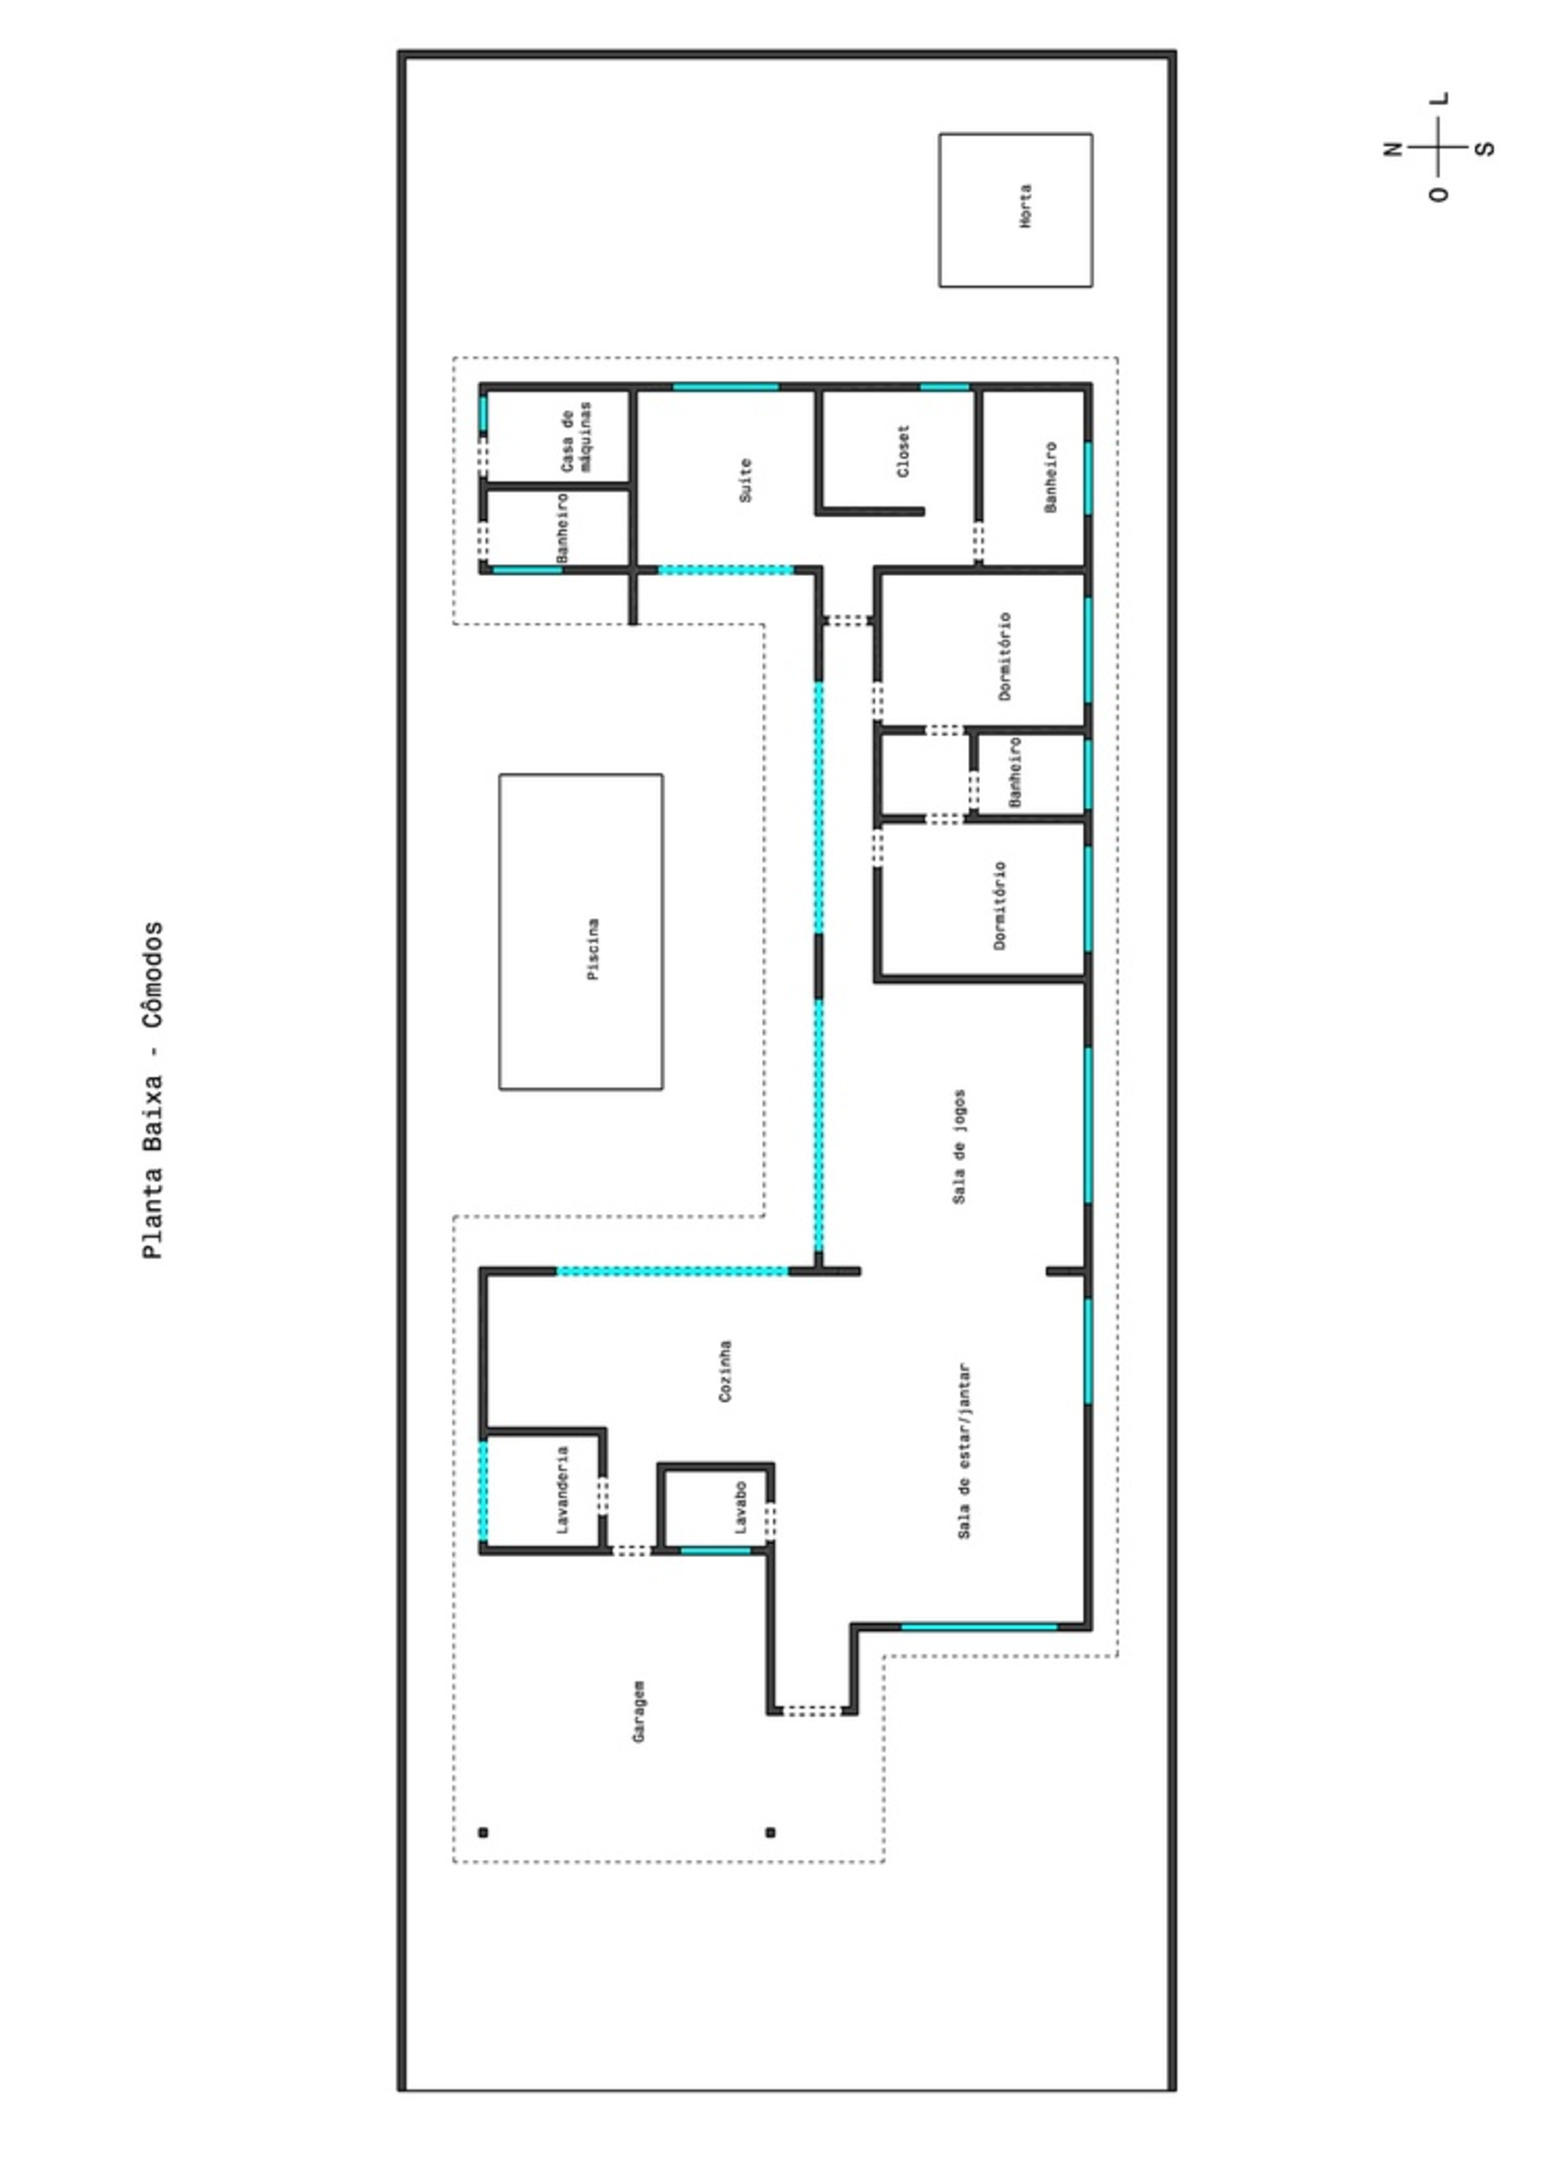
\includegraphics[keepaspectratio,scale=0.45,angle=270]{figuras/planta_comodos.eps}
	\caption{Planta baixa da casa com cômodos}
  \end{center}
\end{figure}

\begin{figure}[H]
  \begin{center}
	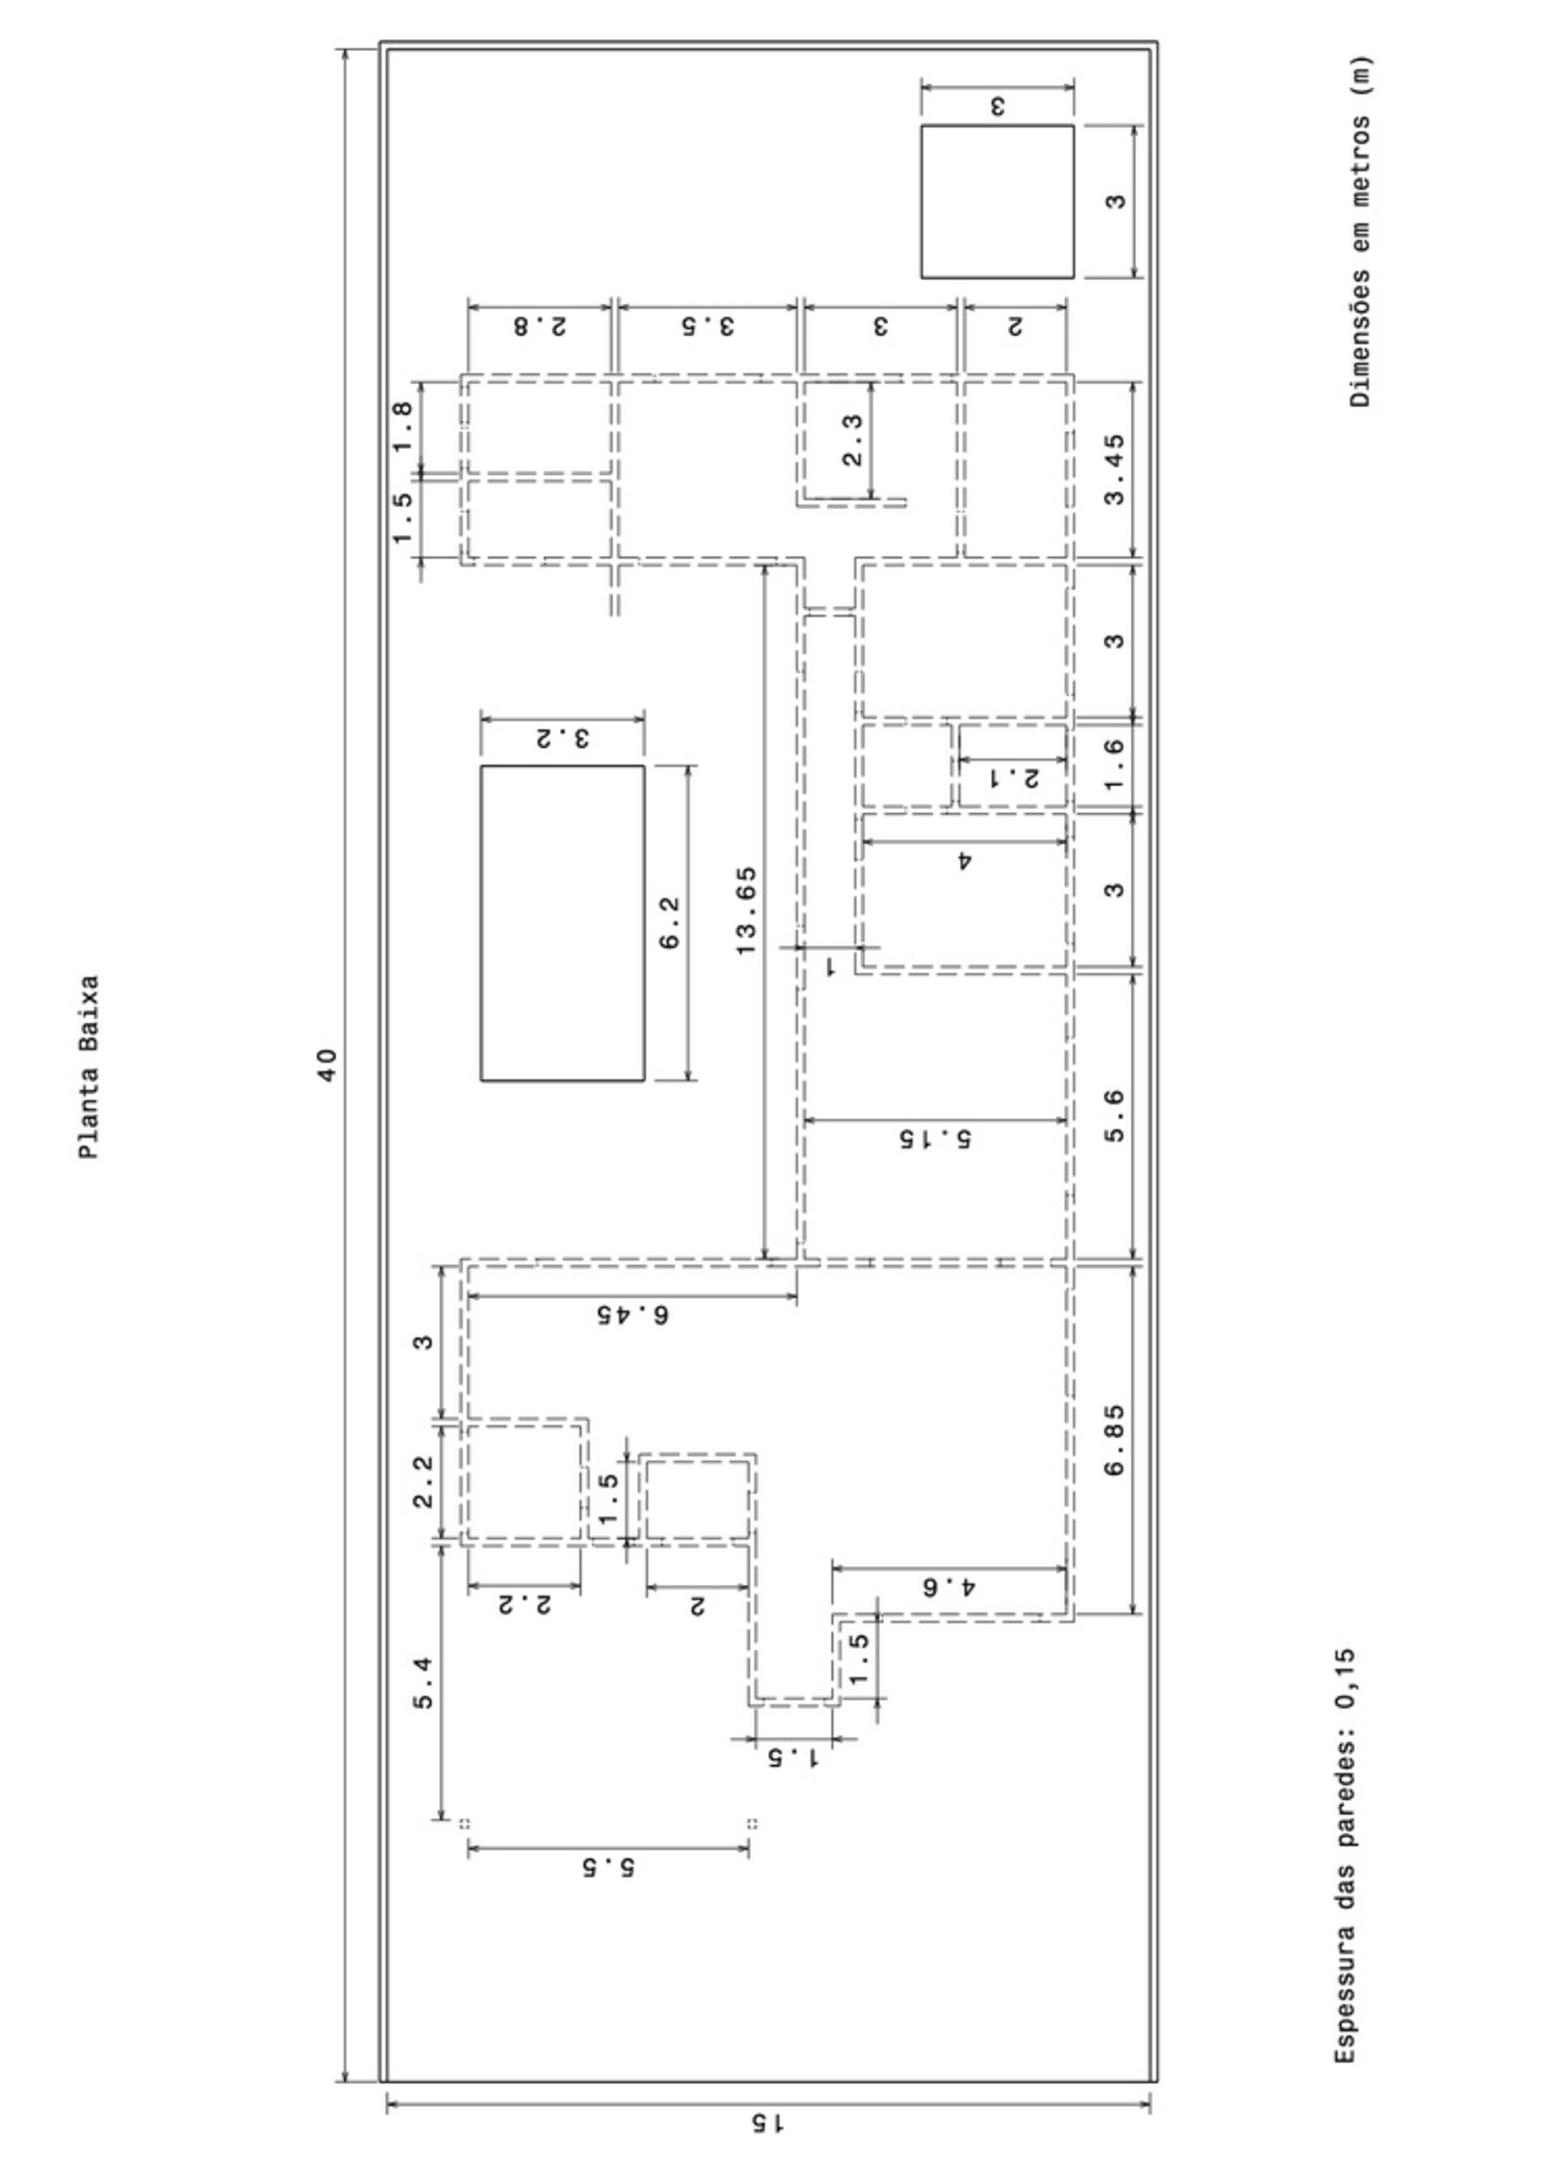
\includegraphics[keepaspectratio,scale=0.45,angle=270]{figuras/planta_baixa.eps}
	\caption{Planta baixa da casa}
  \end{center}
\end{figure}


\subsection{Telhado}

Segundo um dos fabricantes, a inclinação para maior conforto térmico é de 27\%, o que corresponde a aproximadamente $15,66^o$ de inclinação. Esta inclinação converge com a inclinação ótima para a obtenção de energia por meio das placas fotovoltáicas, cuja inclinação com face norte deve corresponder à da latitude para maior eficiência. Portanto conclui-se que $15^o$ de inclinação com a face voltada para o Norte privilegia a captação de energia solar ao mesmo tempo que atende aos requisitos da Telha Ecológica\cite{2013Onduline}\cite{2013Portal}.

A partir destas especificações foi elaborada uma renderização 3D da casa.
\newpage

\begin{figure}[H]
  \begin{center}
	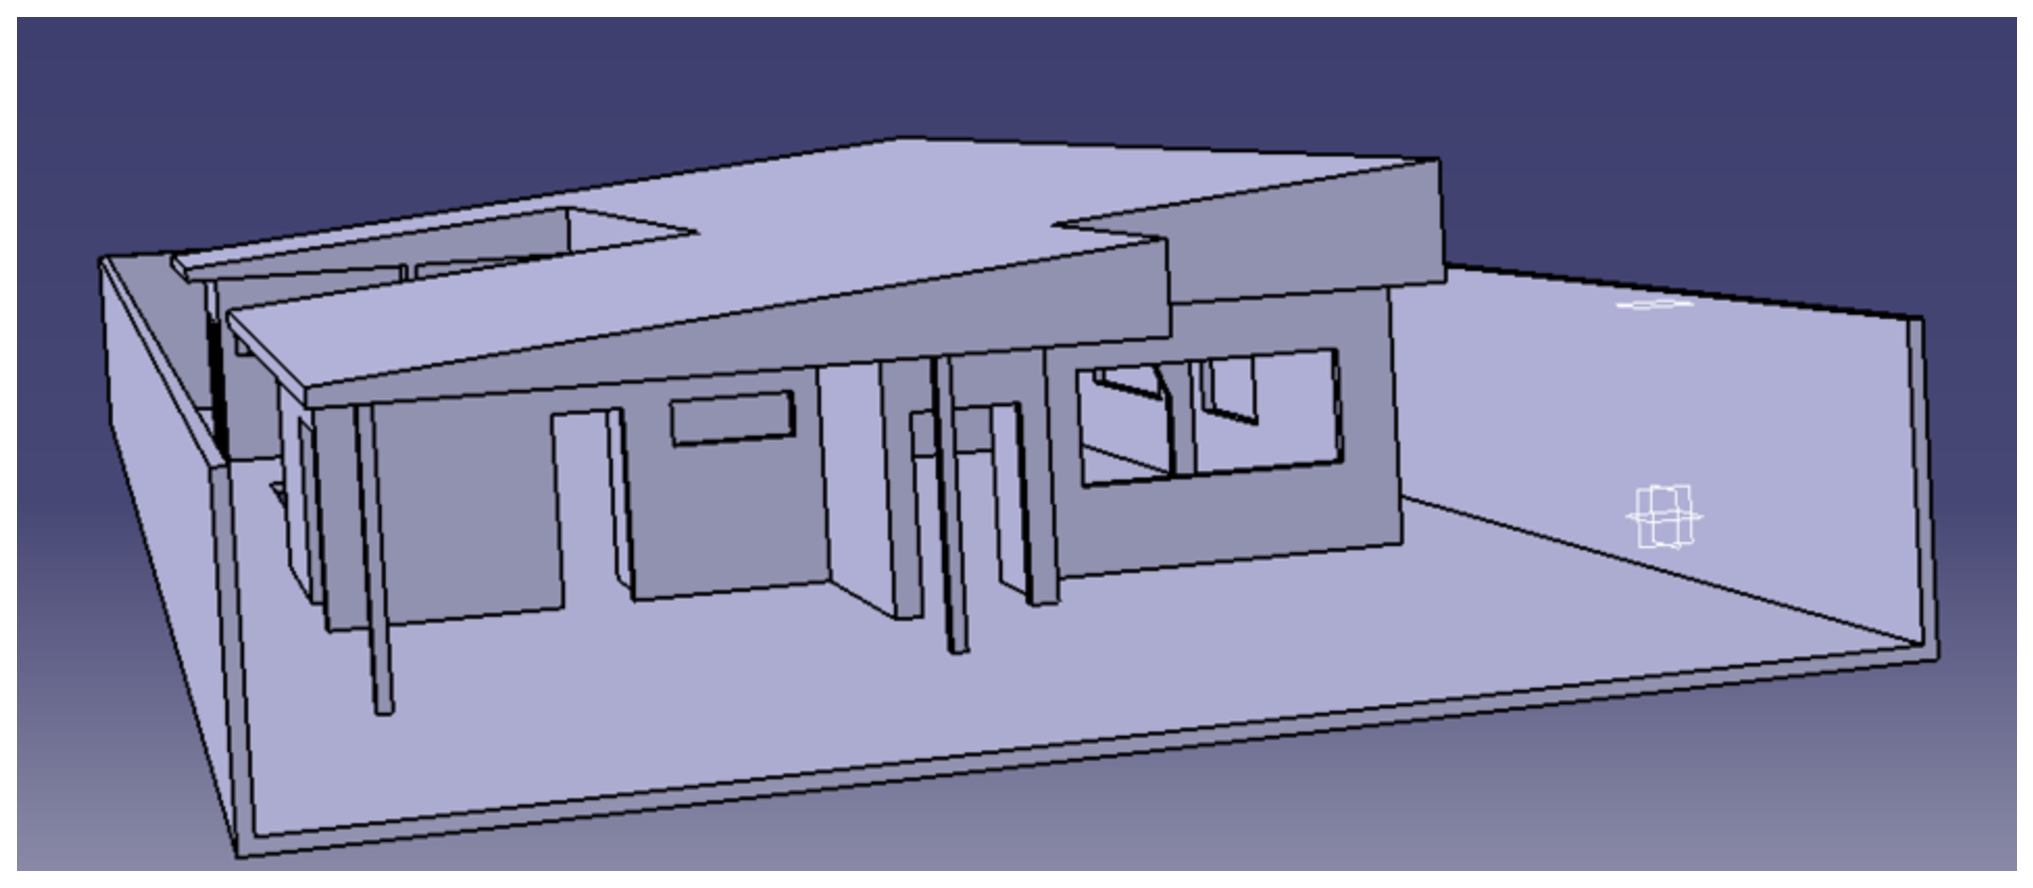
\includegraphics[keepaspectratio,scale=0.5,angle=0]{figuras/3d.eps}
	\caption{Renderização 3D da casa}
  \end{center}
\end{figure}













